\documentclass[a4paper]{article}
\usepackage[utf8]{inputenc}
\usepackage{soul, dingbat}
\usepackage{amsfonts, amsmath, amssymb}
\usepackage{bm}
\usepackage{url}
\usepackage{parskip}
\usepackage{cancel}
\usepackage{upgreek}

% \usepackage[charter]{mathdesign}
\renewcommand*\rmdefault{bch}

\usepackage{geometry}
\geometry{a4paper, 
					left=2.50cm,
					right=2.50cm,
					top=2.50cm,
 					bottom=3.00cm}

\usepackage[usenames,dvipsnames]{xcolor}
\usepackage{hyperref}
\hypersetup{
%	hyperindex,
	breaklinks,
	colorlinks=true,
	linkcolor=blue,
	citecolor=Purple,%	allcolors=black,
	pdfauthor={AOMSS participants},
	pdftitle={AOMSS 2019 Handbook}
}

\usepackage{microtype}
\usepackage{graphicx}

\graphicspath{{figures/}}

\numberwithin{equation}{section}
\numberwithin{figure}{section}

\title{Advanced Ocean Modelling \st{Summer}\footnote{Navid suggests that we remove the word ``Summer'' from the title since late April--early May is not considered summer anywhere in the globe. Madi asks: is a summer school more than just a school that occurs in summer? Perhaps we could leave summer there, crossed out. Navid replies: Of course a `summer school' is more than something that occurs in summer but I think `occurring in summer' is a requirement... Otherwise why not call it `Mars school' or `Ski Retreat' or what not... :) I do like the \st{Summer} proposal though. Madi: Let's have a ski retreat next time. \rightthumbsup}\ \ School 2019:\\Lecture Notes}
\author{AOM\st{S}S participants}
\date{May 2019}

\usepackage{natbib}
\usepackage{graphicx}

\begin{document}

\maketitle

\section*{What's this document about}

This document collates lecture notes from AOM\st{S}S 2019, held at the Lake Pedder Wilderness lodge, April 28th -- May 3rd.

\vspace{1em}

What follows is a list of the subjects of the lectures given along side with the names of those who put their hands up to write up the corresponding notes. The list should be read as:

\vspace{1em}

Lecture Theme (Lecturer; day) --- \textbf{who is writing the notes}

\vspace{2em}

\subsection*{Table of Contents}

\begin{enumerate}
    \item Mass conservation \& Tracer budgets (Steve; Sun + Mon morning) --- \textbf{}
    \item Diffusion equation (Steve; Mon) --- \textbf{???}
    \item Dynamics (Rotating reference frame, hydrostatic--Boussinesq--traditional approximations (Andy; Mon) --- \textbf{Wilma}
    \item Advection equation (Steve; Mon) --- \textbf{Denise}
    \item Reduced gravity model (Andy; Mon) --- \textbf{Stefan}
    \item Tensors and index notation (Navid; Mon) --- \textbf{Ole}
    \item Numerics: Time-stepping schemes (Andy; Tue) --- \textbf{Xihan}
    \item Kinematic boundary conditions / Dynamic \& Permeable surfaces (Steve; Tue) --- \textbf{Mainak}
    \item Numerics: spatial discretisation (Andy; Tue) --- \textbf{Stefan}
    \item Generalised vertical coordinates: kinematic boundary conditions (Steve; Tue) --- \textbf{???}
    \item Generalised vertical coordinates: calculus with GVCs (Steve; Tue) --- \textbf{Chris}
    \item A special GVC: isopycnal coordinates: The hydrostatic, Boussinesq, primitive eqs in isopycnal coords (Andy; Tue + Wed morning) --- \textbf{???}
    \item More GVCs: Diasurface transport (Steve; Wed) --- \textbf{Eva}
    \item Mass continuity in GVCs (Steve; Wed) --- \textbf{Emilio}
    \item Arbirtrary Lagrangian Eulerian scheme (Andy; Wed) --- \textbf{Christelle}
    \item Form drag (kidding... form \textbf{stress}) + exercise (Andy; Wed) --- \textbf{Luwei}
    \item Subgrid Scales in Tracer eq. (Steve; Wed) --- \textbf{???}
    \item Gent--McWilliams parametrisation + exercise (Steve; Wed + Thu) --- \textbf{Josu\'e}
    \item Friction and Stress in models (Andy; Thu) --- \textbf{Dave Gwyther \& Craig Stewart}
    \item Boundary fluxes \& KPP black magic [ha!] (Steve; Thu) --- \textbf{Fabio}
    \item Advection Schemes and Numerical Diffusion (Ryan; Fri) --- \textbf{Ryan}
    \item Available Potential Energy (Andy; Fri) --- \textbf{Danielle}
    \item Numerics: Barotropic--Baroclinic time-stepping split (Steve; Fri) --- \textbf{Madi}
    \item Water mass transformations (Steve; Fri) ---\textbf{Denise}
\end{enumerate}

\newpage

\tableofcontents

\newpage


 % !TEX root = main.tex

\section*{Lecture 0: Writing guidelines and more}
\begin{flushright}\textbf{[by Navid]}\end{flushright}


\subsection*{Note-writing Guidelines}


Please try to stick to the following guidelines while writing your notes.

\begin{itemize}

\item 
Use Australian spelling.

\item
All equations should be numbered, like this one:
\begin{equation}
  \frac{\partial\rho}{\partial t} = \boldsymbol{\nabla}\cdot\boldsymbol{v}.
\end{equation}

\item
Equations should read as prose, i.e., they should be punctuated. (Have a look at this entertaining little piece by Mermin regarding combining equations in text:
\begin{quote}
  N. D. Mermin. What's wrong with these equations? \emph{Phys. Today}, \textbf{42(10)}, 9–11, 1989.\\(Available online at \href{http://www.pamitc.org/documents/mermin.pdf}{http://www.pamitc.org/documents/mermin.pdf}.)
\end{quote}

\item
You can colour text \textcolor{red}{like this} using \verb"\textcolor{color}{text}". Please resist overdoing it though.

\item
Vectors are denoted with \textbf{bold} using \verb"\boldsymbol{...}".

\item
Notation is as follows:
\begin{align}
 \text{horizontal velocity field:}\quad &\boldsymbol{u} = (u, v), \\
 \text{three-dimensional velocity field:}\quad &\boldsymbol{v} = (u, v, w),\\
 &\ \ \vdots \nonumber
\end{align}

\item
Let's use $\times$ for cross products, e.g., $[\boldsymbol{a}\times\boldsymbol{b}]_i = \epsilon_{ijk}a_jb_k$.

\item
Since these are notes, it might be useful to cross out term in equations as, e.g., 
\begin{equation}
    \cancel{x} + 5 + y  = \cancel{x}.
\end{equation}

\item
Fourier transformed variables should be denoted with hats:
\begin{equation}
    \boldsymbol{u}(\boldsymbol{x}) = \sum_{\boldsymbol{k}} \hat{\boldsymbol{u}}_{\boldsymbol{k}} e^{i \boldsymbol{x}\cdot\boldsymbol{k}}.
\end{equation}

\item
Partial derivatives should be either written in full, e.g., $\partial\rho/\partial t$ or as $\partial_t\rho$ but \emph{\bf not} using $\rho_t$ notation.

\item
Andy used in places subscript-comma notation to denote partial derivatives, e.g., $\partial_y u = u_{,2}$. Since this notation was not widely spread throughout the lectures, let's just stick to the usual $\partial_y u$.

\item
Add figure files in the \verb"figures/" folder and then incorporate them in the text using the usual 
\begin{quote}
    \verb"\begin{figure}"\\
    ...\\
    \verb"\end{figure}"
\end{quote}
environment with \verb"\includegraphics[width=3in]{figurename}". Note that you need not include the figure's folder path, e.g., \verb"\includegraphics[width=3in]{figures/figurename}".

\item
Hand-drawn figs/diagrams are mostly welcome!

\item
Refrain from using $\cdot$ or $\times$ for plain multiplication (except when it's absolutely necessary to avoid ambiguity)! Symbol $\cdot$ (\verb"\cdot") should only denote a dot product, while $\times$ (\verb"\times") should only denote a cross product.

\end{itemize}

\begin{figure}[h!]
  \centering
  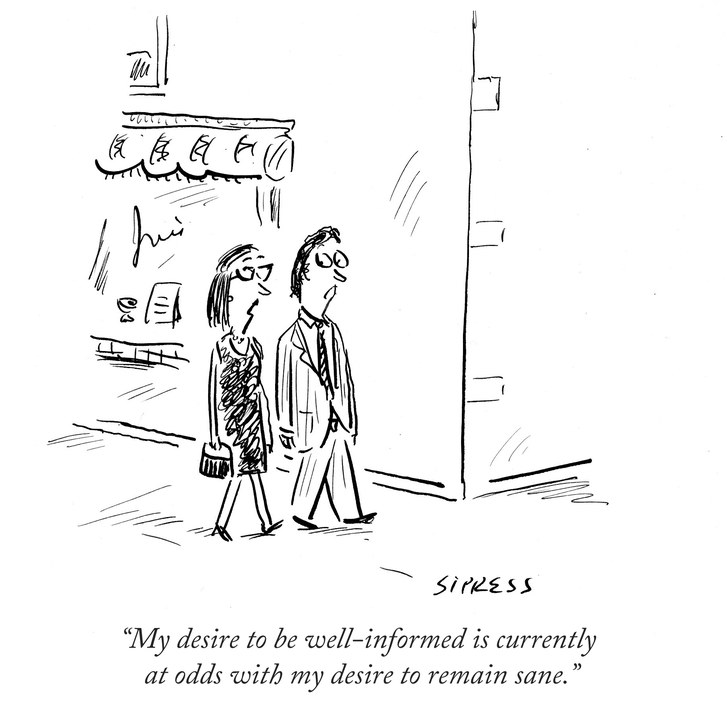
\includegraphics[width=3in]{newyorkercomic}
  \caption{A caption is often useful.}
\end{figure}


% !TEX root = main.tex

\section{Lecture 1: Title goes here}
\begin{flushright}\textbf{[by ????]}\end{flushright}


% !TEX root = main.tex

\section{Lecture 2: Rotate the planet}\label{sec:lecture2}
\begin{flushright}\textbf{[by Annie]}\end{flushright}
  
 \begin{itemize}
   \item
   How rotation changes things
   \item
   Touch on: Geostrophy, Thermal wind
   
\end{itemize}

% !TEX root = main.tex

\section{Lecture 3: Dynamics}
\begin{flushright}\textbf{[by Wilma Huneke]}\end{flushright}

{\color{red}Navid: Wilma, I added some notes/remarks with red.}
%Rotating reference frame, hydrostatic - Boussinesq - traditional approximations\\
\textcolor{red}{Wilma: Might add some figures later.}

We start with the mass and momentum equations, the latter is also known as the Navier-Stokes equation:

\begin{gather}
\frac{D\rho}{Dt} + \rho\boldsymbol{\nabla} \cdot \boldsymbol{v} = 0,
\label{Eq:mass} \\
\frac{D\boldsymbol{v}}{Dt} = \underbrace{\frac{\partial \boldsymbol{v}}{\partial t}}_{\text{change in time}} + \underbrace{\left( \boldsymbol{v}\cdot \boldsymbol{\nabla}\right)\boldsymbol{v}}_{\text{adv. of momentum}} = \underbrace{\boldsymbol{g}}_{\text{grav. accel.}} - \underbrace{\frac{\boldsymbol{\nabla} p}{\rho}}_{\text{pressure gradient}} + \underbrace{\nu\nabla^2 \boldsymbol{v}}_{\text{viscous term}},
\label{Eq:NS}
\end{gather}
where the gravitational acceleration is defined as $\boldsymbol{g}= (0,0,-g)$.
The assumptions that went into the above equations are conservation of mass (equation \ref{Eq:mass}) and conservation of momentum (equation \ref{Eq:NS}). The Navier-Stokes equation additionally assumes a Newtonian fluid, which means the viscous transfer of momentum is linear (non-Newtonian fluids such as ice require a representation of viscosity in tensor form). For a detailed derivation of equations \ref{Eq:mass} and \ref{Eq:NS} see, e.g., \citet{Griffies2019}, chapter 26.

%{\color{red}Navid: Wilma, could you punctuate equations? Equations should be read as prose so commas, periods, or even question marks should appear after them...}

In order to make the dynamic equations useful for ocean modelling, we have
\begin{enumerate}
\item to add Coriolis: take into account that we are in rotating reference frame (and do the so-called `traditional approximation'), 
\item to do the hydrostatic approximation, and
\item to do the Boussinesq approximation.
\end{enumerate}

It is important to keep in mind what we omit in steps 1-3 above!

\subsection{Rotating reference frame}
Equations \ref{Eq:mass} and \ref{Eq:NS} are given in a fixed reference frame. Let us translate the fixed frame to a rotating frame. We define

\begin{equation}
\begin{aligned}
\boldsymbol{v}_f &= \frac{d_f\boldsymbol{x}}{dt} \qquad \text{fixed frame velocity,}\\
\boldsymbol{v}_r &= \frac{d_r\boldsymbol{x}}{dt} \qquad \text{rotating frame velocity,}\\
\end{aligned}
\end{equation}
and translate between the two frames
\begin{equation}
\frac{d_f\boldsymbol{x}}{dt} = \frac{d_r\boldsymbol{x}}{dt} + \boldsymbol{\Omega} \times \boldsymbol{x}.
\label{Eq:fi-ro}
\end{equation}

Now, let's repeat the process once more, this time for the velocity vector:
\begin{equation}
\begin{aligned}
\frac{d_f\boldsymbol{v}}{dt} &= \frac{d_r\boldsymbol{v}_f}{dt} + \boldsymbol{\Omega} \times \boldsymbol{v}_f\\
& = \frac{d_r}{dt}\left[\frac{d_f\boldsymbol{x}}{dt}\right]+ \boldsymbol{\Omega} \times \frac{d_f\boldsymbol{x}}{dt} \qquad \implies \text{expand using } (\ref{Eq:fi-ro}) \\
& = \frac{d_r}{dt}\left[ \frac{d_r\boldsymbol{x}}{dt} + \boldsymbol{\Omega} \times \boldsymbol{x} \right] + \boldsymbol{\Omega} \times \left[ \frac{d_r\boldsymbol{x}}{dt} + \boldsymbol{\Omega} \times \boldsymbol{x}  \right].
\end{aligned}
\end{equation}


Thus, gathering everything together we get:
\begin{equation}
\underbrace{\frac{d_f\boldsymbol{v}}{dt} }_{\text{fixed}} = \underbrace{\frac{d_r\boldsymbol{v}_r}{dt} + 2\boldsymbol{\Omega} \times \boldsymbol{v}_r + \boldsymbol{\Omega}\times (\boldsymbol{\Omega} \times \boldsymbol{x})}_{\text{rotating frame}}.
\end{equation}

We can now rewrite the Navier-Stokes equation in a rotating framework:
\begin{equation}
\frac{D\boldsymbol{v}}{Dt} + \underbrace{2 \boldsymbol{\Omega} \times \boldsymbol{v}}_{\#2} + \underbrace{\boldsymbol{\Omega} \times (\boldsymbol{\Omega} \times \boldsymbol{x})}_{\#1} = \boldsymbol{g} - \frac{\boldsymbol{\nabla} p}{\rho} + \nu \nabla^2 \boldsymbol{v},
\end{equation}
where we use from now on the rotating frame velocity.

Let us have a closer look at the two new terms appearing in the rotating framework.

\subsubsection*{\#1: $\qquad \boldsymbol{\Omega} \times (\boldsymbol{\Omega} \times \boldsymbol{x}) = -\boldsymbol{r} |\boldsymbol{\Omega}|^2 \qquad$ Centrifugal force}

The centrifugal force is a body force and depends only on the distance $\boldsymbol{r}$ from the rotation axis (this is not the Earth radius!) and the rotation rate. {\color{red}[Navid: A figure would be useful here. E.g., one might wonder where is $\boldsymbol{r}$ pointing?]} We can combine the centrifugal force with the gravitational acceleration (gravity force) and write
\begin{equation}
\boldsymbol{g}* = \boldsymbol{g} + \boldsymbol{r}\Omega^2,
\end{equation}
where $|\boldsymbol{\Omega}|^2 = \Omega^2$. %{\color{red}[Navid: This is not an approximation, this is exactly the definition of the modulus of $\boldsymbol{\Omega}$. The $\approx$ should be simply an $=$. Is there a different approximation that was used in getting (3.8)?]} 

{\color{red} Navid: I added this small exercise.}

\noindent\textbf{Exercise:} Prove identity $\boldsymbol{\Omega} \times (\boldsymbol{\Omega} \times \boldsymbol{x}) = -\boldsymbol{r} |\boldsymbol{\Omega}|^2$. (Hint: Index notation (which is introduced in  lecture~\ref{sec:tensors})   proves to be very helpful here.)

When we plug in typical values for the equator ($r\approx 10^6$ m, $\Omega \approx 10^{-4}$ s$^{-1}$, $g \approx 10$ m\,s$^{-1}$), we can see that $r\Omega^2\approx0.05$ is smaller than $\boldsymbol{g}$, but not completely negligible. Therefore, the $\boldsymbol{r}\Omega^2$ is not dropped, but for simplicity the resultant force is often called gravitational force and the asterisk is dropped. 

We now write the combined gravity force and centrifugal force term in potential form:
\begin{align}
\boldsymbol{g}*& = \begin{pmatrix}
0\\0\\-g
\end{pmatrix} + \boldsymbol{r}\Omega^2 \nonumber\\
& = \boldsymbol{\nabla}\left[ -g z + \frac{r^2\Omega}{2} \right] \nonumber\\
& = \boldsymbol{\Omega} \Phi,
\end{align}
where $\Phi$ is called the `geopotential'.

Be aware that we ignore the moon gravitation (tides -- one way to implement them in models is in the gravity force term) and ice sheet gravitation. We also assume the Earth is a perfect sphere. These all affect $\boldsymbol{g}$ as well.

\subsubsection*{\#2 $\qquad 2 \boldsymbol{\Omega} \times \boldsymbol{v}$ \qquad Coriolis force}

Let us take the cross product of the Coriolis term and write
\begin{align}
2\boldsymbol{\Omega}\times\boldsymbol{v} & = \begin{vmatrix}
\hat{\boldsymbol{x}} & \hat{\boldsymbol{y}} & \hat{\boldsymbol{z}} \\
0 & 2\Omega\cos\phi & 2\Omega\sin\phi\\
u & v & w
\end{vmatrix} \nonumber\\
& =  (2 \Omega w \cos\phi - 2\Omega v \sin\phi )\hat{\boldsymbol{x}} +  (2\Omega u \sin \phi)\hat{\boldsymbol{y}} +  (-2 \Omega u \cos \phi)\hat{\boldsymbol{z}} \nonumber\\
& = (-\tilde{f}w - fv)\hat{\boldsymbol{x}} + fu \hat{\boldsymbol{y}} - \tilde{f}u \hat{\boldsymbol{z}},
\end{align}
where we have defined:
\begin{equation}
\begin{aligned}
f &= 2\Omega\sin\phi \qquad \text{traditional Coriolis term, and} \\
\tilde{f} &= 2\Omega\cos\phi \qquad \text{non-traditional Coriolis term.} \\
\end{aligned}
\end{equation}

%{\color{red}[Isn't this notation for (3.11) better? What do you think?]}

{\color{red}[Navid: Again, a figure here might be useful to clarify that $\hat{\boldsymbol{x}}, \hat{\boldsymbol{y}}$ are the locally horizontal unit vectors and $\hat{\boldsymbol{z}}$ the locally vertical unit vector.]}

Most models use only the traditional Coriolis term in the momentum equation, as the following subsection will explain.


\subsection{Hydrostatic approximation}
Let us have a look at the vertical component of the Navier-Stokes equation, taking the Coriolis term into account:

\begin{equation}
\frac{\partial w}{\partial t} + (\boldsymbol{v}\cdot \boldsymbol{\nabla})w -\tilde{f}u = -g -\frac{1}{\rho} \frac{\partial p}{\partial z} + \nu \nabla^2w
\label{Eq:VertMom}
\end{equation}

A scaling analysis {\color{red}(i.e., plugging in typical values for the various terms)} reveals that the dominant balance in the above equation \ref{Eq:VertMom} comes between the pressure term and gravity:
{\color{red}[Navid: Sorry, I had to be more specific... What I meant is to write up 1-2 sentences explaining that, e.g., if we are interested for motions that involve down to mesoscale eddies then  horizontal length scales are ... km, a velocity scale is .... m/s and therefore.....]}
%Terms that are neglected in the hydrostatic approximation:
\begin{equation}
\begin{aligned}
\frac{\partial w}{\partial t} \qquad &\rightarrow \frac{10^{-3}}{10^5} = 10^{-8}\\
(\boldsymbol{v}\cdot \boldsymbol{\nabla})w \qquad &\rightarrow \frac{1}{10^{4}} 10^{-3} = 10^{-7}\\
\tilde{f}u \qquad &\rightarrow 10^{-5}\\
\nu \nabla^2w \qquad &\rightarrow \text{small} \\
\hline
g \qquad &\rightarrow 10
\end{aligned}
\label{Eq:HydrScale}
\end{equation}

The balance between pressure and gravity is the so-called `hydrostatic pressure balance' and it allows us to simplify the vertical momentum equation to

\begin{equation}
\frac{\partial p}{\partial z} = - \rho g.
\end{equation}

%{\color{red}[Navid: Wilma I think you should first do the scalings and show how (3.12) reduces to (3.13) and then proceed with the the comments below on no-prognostic eq. for $w$, etc. What do you reckon?}

Thus, the hydrostatic approximation removes the vertical velocity $w$ as a prognostic variable (no $\frac{\partial w}{\partial t} = ...$). A non-hydrostatic model retains the full vertical momentum equation and $w$ as a prognostic variable. 

The above scalings \ref{Eq:HydrScale} allow us to discard the vertical component in the Coriolis force
\begin{equation}
2\boldsymbol{\Omega} \times \boldsymbol{v} \approx (\tilde{f}w - fv)\hat{\boldsymbol{x}}  + fu \hat{\boldsymbol{y} } .
\end{equation}

Furthermore, a similar scaling argument when comparing $w< 10^{-3}$ ms$^{-1}$ with $v=1$ ms$^{-1}$ allows us to discard the non-traditional Coriolis term in the $x$-component of the Coriolis term, known as the traditional approximation. Hydrostatic models therefore only make use of the traditional Coriolis term.

Quasi non-hydrostatic models retain the $\tilde{f}u$ term and have a balance between
\begin{equation}
\tilde{f}u = -g -\frac{1}{\rho}\frac{\partial p}{\partial z}.
\end{equation}

To sum up, the hydrostatic approximation emphasises the strong effect that gravity has on the direction it acts on. The hydrostatic approximation is computationally advantageous as it reduces the number of prognostic variables our model needs to evolve. However, we need to remember that it holds only when the horizontal velocities are much larger than the vertical velocities (rule of thumb: horizontal length scales $\approx$ 10 km vs vertical length scale $\approx$ 10 m). Internal waves can be resolved in a hydrostatic model, but they cannot overturn. Hydrostatic models are, therefore, not a useful tool to study turbulent processes for which the ratio of the horizontal and vertical scales become equal. Quasi non-hydrostatic models retain the non-traditional Coriolis term, but suffer under increased computational costs.

\subsection{Boussinesq approximation}
The Boussinesq approximation assumes the ocean is an incompressible fluid and ignores density fluctuations except in the gravity term.

The mass conservation equation \ref{Eq:mass} reduces to
\begin{equation}
\cancel{\frac{D\rho}{Dt}} + \rho \boldsymbol{\nabla} \cdot \boldsymbol{v} = 0 \Longrightarrow  \boldsymbol{\nabla} \cdot \boldsymbol{v} = 0 \qquad \text{(conservation of mass, incompressibility).} \label{incompressibility}
\end{equation}

From \eqref{incompressibility} above we can obtain a diagnostic equation for $w$:
\begin{equation}
 \frac{\partial u}{\partial x} + \frac{\partial v}{\partial y} + \frac{\partial w}{\partial z} = 0 \Longrightarrow
 \frac{\partial w}{\partial z} = -\frac{\partial u}{\partial x} - \frac{\partial v}{\partial y}.
\end{equation}

Therefore, the horizontal momentum equations reduce to
\begin{equation}
\begin{aligned}
\frac{\partial u}{\partial t} + u\frac{\partial u}{\partial x} + v\frac{\partial u}{\partial y} + w\frac{\partial u}{\partial z} -fv &= -\frac{1}{\rho_0} \frac{\partial p}{\partial x} + \nu \nabla^2 u, \\
\frac{\partial v}{\partial t} + u\frac{\partial v}{\partial x} + v\frac{\partial v}{\partial y} + w\frac{\partial v}{\partial z} +fu &= -\frac{1}{\rho_0} \frac{\partial p}{\partial x} + \nu \nabla^2 u.
\end{aligned}
\end{equation}

Remarks: 
\begin{itemize}
\item The density $\rho_0$ in the pressure term is a constant reference density. Be careful as the subscript 0 is often omitted for simplicity.
\item The ocean density $\rho = f(S, T, p)$ can still change and produce a pressure gradient. The Boussinesq approximation assumes, however, that $\rho$ does not change due to compressibility of the fluid.
\item The Boussinesq approximation filters out sound waves from the equations as they require density fluctuations to propagate.
\item The Boussinesq approximation gives as a simple diagnostic equation for the vertical velocity based on the mass conservation equation. Non-incompressible models have a more complicated form of the diagnostic equation (but it is still diagnostic as long as the model is hydrostatic).
\item The horizontal momentum equations still have $w$ and with it vertical advection. 
\end{itemize} 

% !TEX root = main.tex

\section{Lecture 4: The advection Equation (and some related jargon)}
\begin{flushright}\textbf{[by Denise Fernandez]}\end{flushright}

We have discussed the diffusion equation in Lecture~\ref{sec:lecture2}, where we considered the difference between the random molecular motion versus the motion of the centre of mass of all constituents of a fluid. Here ``advection" refers to the movement of fluid from place to place in reversible physical processes while diffusion considers irreversible exchanges and mixing processes where the matter content and thermodynamics of a fluid element are altered \citep{Griffies2019}. 

In this lecture we consider the macroscopic motion of a fluid element. The material derivative of the tracer concentration $C$ of the fluid remains constant as the element moves with the fluid (Fig. \ref{fig:trajC}), that is $C(\boldsymbol{x},t)= C[\boldsymbol{x}(0)]$ and 

\begin{equation}
    \frac{\mathrm{D}C}{\mathrm{D}t}= \frac{\partial C}{\partial t} + \boldsymbol{v} \cdot \boldsymbol{\nabla} C = 0.
    \label{Eq:adv1}
\end{equation}

\begin{figure}[h]
\centering
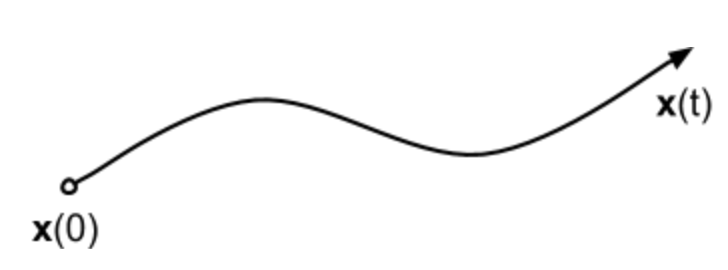
\includegraphics[width=0.3\textwidth]{figures/Lecture4_fig1.png}
\caption{Trajectory of the tracer concentration $C$ with no diffusion, just transport of the particle.}
\label{fig:trajC}
\end{figure}

Here we use the chain rule and the constancy of the tracer concentration to show that advection of the transport concentration is reversible,

\begin{equation}
    \frac{DC}{Dt}^{\alpha} = C ^{\alpha -1} \frac{DC}{Dt} = 0.
    \label{Eq:adv2}
\end{equation}

where $\alpha$ is an arbitrary number. 
\subsection{Mass transport from the mean, eddy and residual mean}

The density $\rho$ is an example of such a tracer and evolves according to:
\begin{equation}
    \frac{\partial \rho}{\partial t}= -\boldsymbol{\nabla} \cdot (\boldsymbol{v}\rho).
    \label{Eq:tend1}
\end{equation}

The mass density time tendency (i.e., $\partial \rho/\partial t$) remains unchanged if the advective mass flux $\rho \boldsymbol{v}$ is modified by the addition of the eddy-induced mass flux of the form $\rho\boldsymbol{v}^* = \boldsymbol{\nabla}\times(\rho\boldsymbol{\Psi})$ (where $\boldsymbol{\Psi}$ is a vector streamfunction),
\begin{align}
    \boldsymbol{v} \rho \rightarrow \boldsymbol{v}^\dagger \rho &\equiv (\boldsymbol{v} + \boldsymbol{v}^*) \rho \\
    & = \rho \boldsymbol{v} + \rho \boldsymbol{v}^*,\\
    & = \rho \boldsymbol{v} + \boldsymbol{\nabla}\times(\rho\boldsymbol{\Psi}).
        \label{Eq:add_massflx}
\end{align}

The additional mass flux $\boldsymbol{\nabla} \times (\rho \boldsymbol{\Psi}$) in Eq. \eqref{Eq:add_massflx} does not lead to accumulation of mass since its divergence is zero. This is known as ``Gauge Invariance" symmetry resulting from the decomposition of the mass flux into a mean and a non-divergent fluctuation \citep{Griffies2019}. 


The terminology is the following: %I'd like to add subequations..
\begin{subequations} %Here's how you add subequations. Awesome, thanks!
\begin{align}
    \boldsymbol{v} &= \text{Eulerian mean velocity}, \\
    \rho \boldsymbol{v} &= \text{Eulerian mean mass flux (per unit volume)}, \\
    \boldsymbol{v}^* &= \text{Eddy-induced velocity}, \\
    \rho \boldsymbol{v}^* &= \boldsymbol{\nabla} \times (\rho \boldsymbol{\Psi}) = \text{Eddy-induced mass flux}, \label{Eq:eddy_mass_flx}\\
    \boldsymbol{v}^\dagger &= \boldsymbol{v}+\boldsymbol{v}^* = \text{Residual mean velocity \space (i.e. winds$+$rotation due to eddies)}, \\
    \rho \boldsymbol{v}^\dagger &= \text{Residual mean mass flux}. 
 \end{align} 
 \end{subequations}
 
Now we turn into the tracer advection equation to derive the eddy Skew flux. 

Consider the transport concentration is determined by the residual velocity (remember: the ``eddy contribution often compensates for the mean, with sum of the mean and eddy representing a residual" \citep{Griffies2019}),
 
 \begin{equation}
     \frac{\partial (\rho C)}{\partial t} + \boldsymbol{\nabla} \cdot (\rho \boldsymbol{v}^\dagger C) = 0.
     \label{Eq:TAEq}
 \end{equation}
 
 Using Eq. \eqref{Eq:eddy_mass_flx} for the eddy-induced mass flux and the tracer advection equation with the advective transport determined by the residual mean velocity (Eq.~\eqref{Eq:TAEq}) we can write 
 \begin{align}
      \rho \boldsymbol{v}^\dagger C &= C(\rho \boldsymbol{v} + \rho \boldsymbol{v}^*) \nonumber\\
    																& = C\rho \boldsymbol{v} + C \boldsymbol{\nabla} \times (\rho \boldsymbol{\Psi}) \nonumber\\
    																&= C\rho \boldsymbol{v} + \boldsymbol{\nabla} \times (C \rho \boldsymbol{\Psi}) - \boldsymbol{\nabla} C \times \boldsymbol{\Psi} \rho.
 \end{align}	
 (Above, to go from the second to the third line we just used Leibniz rule for derivatives of products.)

 What matters for the evolution of $\rho C$ is the divergence of the tracer flux
  \begin{equation}
      \boldsymbol{\nabla} \cdot (\rho \boldsymbol{v}^\dagger C) = \boldsymbol{\nabla} \cdot (C\rho \boldsymbol{v}) - \boldsymbol{\nabla} \cdot (\boldsymbol{\nabla} C \times \rho \boldsymbol{\Psi}),
  \end{equation}
  or after bringing the $\boldsymbol{\nabla} \cdot (C\rho \boldsymbol{v})$ on the right-hand side:
  \begin{equation}
      \boldsymbol{\nabla} \cdot (\rho C \boldsymbol{v}^*) =  \boldsymbol{\nabla} \cdot (\underbrace{-\boldsymbol{\nabla} C \times \rho \boldsymbol{\Psi}}_{\text{eddy skew flux}}). \label{eq4.10}
  \end{equation}

Equation~\eqref{eq4.10} implies that 
\begin{equation}
      \substack{\text{\normalsize\textbf{Divergence of}}\\\text{\normalsize\textbf{the eddy advection flux}}} =  
			\substack{\text{\normalsize\textbf{Divergence of}}\\\text{\normalsize\textbf{the eddy skew flux}}}
\end{equation}
 and because the tracer flux does not cross iso-surfaces, that is, $\boldsymbol{\nabla} C \cdot (-\boldsymbol{\nabla} C \times \rho \boldsymbol{\Psi}) = 0$, the flux is \textbf{skew} and oriented parallel to the iso-surfaces of tracer concentration (see figure~\ref{fig:skewF}).


\begin{figure}[h]
\centering
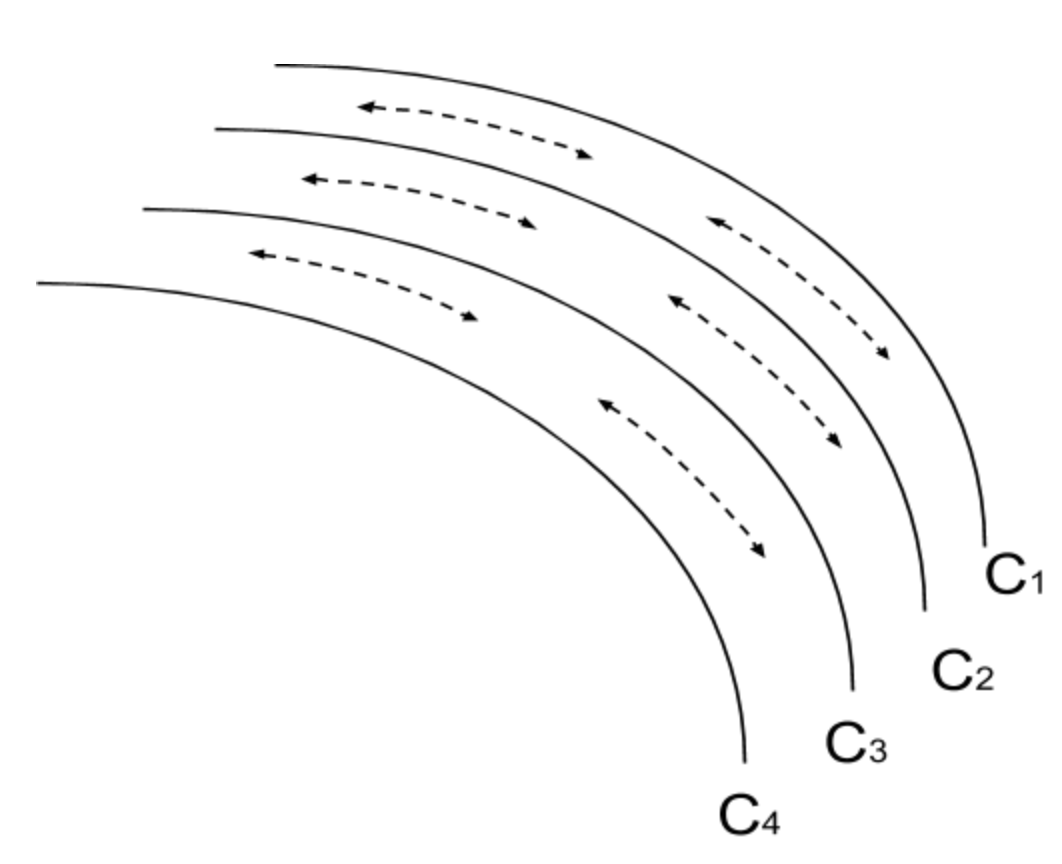
\includegraphics[width=0.3\textwidth]{figures/Lecture4_fig2.png}
\caption{Schematic of the skew fluxes (dashed arrows) for a tracer concentration $C$ parallel to iso-lines of constant $C$ (solid curves).}
\label{fig:skewF}
\end{figure}
 
 \subsection{Skew diffusion}
 {\color{red}[Navid: Andy/Stephen, this sections seems a bit out-of-context here. How should we improve it? Perhaps we should postpone it until the GM lecture?]}

 In tensor notation the advection of the Eddy Skew flux $J^{\textrm{skew}}_m = \big[ -\boldsymbol{\nabla} C \times \rho \boldsymbol{\Psi}\big]_m$ is          
\begin{align}
    J^{\textrm{skew}} _m &= \left( \epsilon_{mnp} \frac{\partial C}{\partial x^n}\right)\rho \Psi_p \\
    & = A_{mn} \frac{\partial C}{\partial x^n}
\end{align}
%ideally use \mathbb
where
\begin{equation}
A_{mn} \equiv \epsilon_{mnp} \Psi_p = \begin{pmatrix}
                                    0 & \Psi_3 & -\Psi_2\\
                                    -\Psi_3 & 0 & \Psi_1\\
                                    \Psi_2 & -\Psi_1 & 0
                                \end{pmatrix},
\end{equation}
is the \textbf{Skew diffusion tensor} and $\epsilon_{mnp}$ the Levi-Civita tensor. (For details and definition of $\epsilon_{mnp}$ refer to Lecture~\ref{sec:tensors}.)
% !TEX root = main.tex

\section{Lecture 5: Axisymmetric circulations}\label{sec:lecture5}
\begin{flushright}\textbf{[by Marty]}\end{flushright}
  
 \begin{itemize}
   \item
   Held \& Hou axisymmetric circulation
   \item
   Eddies
\end{itemize}

% !TEX root = main.tex

\section{Lecture 6: Shallow water}\label{sec:lecture6}
\begin{flushright}\textbf{[by Navid]}\end{flushright}
  
 \begin{itemize}
   \item
   Shallow water dynamics
   \item
   Gravity waves
   \item
   Rossby waves
   \item
   PV?
 \end{itemize}

% !TEX root = main.tex

\section{Lecture 7: Numerics: Time-stepping schemes}
\begin{flushright}\textbf{[by Xihan Zhang]}\end{flushright}

{\color{red}[Navid: Xihan, I made some small editorial comments and added 1-2 explanatory sentences. Have a look and tell me if all is OK.]}

In this lecture, we consider how models time-step forward in time by using finite difference method. 


Take the evolution of thickness $h(\boldsymbol{x}, t)$ in a layered model that was derived in lecture~\ref{sec:lecture5}: 

\begin{equation}
\frac{\partial h}{\partial t}+\frac{\partial (uh)}{\partial x}+\frac{\partial (vh)}{\partial y}=0 .
\label{layereqn}
\end{equation}

Since we want to know how thickness $h$ evolves with time, we rearrange \eqref{layereqn} as 

\begin{equation}
\frac{\partial h}{\partial t}=\underbrace{-\frac{\partial(uh)}{\partial x}-\frac{\partial (vh)}{\partial y}}_{\equiv F(\boldsymbol{x}, t)}.
\label{tmstep}
\end{equation}

We collectively denote all term on the right-hand-side above as $F$.

Now, let's consider a discretization of time into equal increments:
\begin{equation}
	0, \Delta t, 2 \Delta t, \dots, \tau \Delta t, \dots, \label{eq7.3}
\end{equation}
where $\tau$ is an integer. This way the $\tau$-th discrete time corresponds to value $t=\tau\,\Delta t$, $\tau=0,1,\dots$. We denote, hereafter, all field values at $t=\tau\,\Delta t$ simply with a subscript $\tau$, e.g.,
\begin{equation}
	h(\boldsymbol{x}, \tau\,\Delta t) \leftrightarrow h_\tau(\boldsymbol{x}),
\end{equation}
and similarly for $u$, $v$, $F$, etc. Thus, \eqref{tmstep} becomes
\begin{equation}
	\frac{\partial h_\tau}{\partial t} = F_\tau. \label{Ftau}
\end{equation}

What we need to do is to find a way to approximate the time-derivative $\partial h_\tau/\partial t$ on the left-hand-side above within our discrete time-domain~\eqref{eq7.3}.


\subsubsection*{Forward difference time-stepping scheme}

By definition, the continuous version of the time-derivative is:
\begin{equation}
\frac{\partial h_{\tau}}{\partial t}=\displaystyle \lim_{\delta t\to 0}\frac{h(\tau\,\Delta t+\delta t)-h(\tau\,\Delta t)}{\delta t}.
\label{dhdt}
\end{equation}

The discretised approximation of \eqref{dhdt}, after we take $\delta t = \Delta t$, becomes:
\begin{equation}
\frac{\partial h_{\tau}}{\partial t} \approx \frac{h_{\tau +1}-h_{\tau}}{\Delta t}.
\label{dhdt1}
\end{equation}

To obtain the forward step for $h$, combine \eqref{Ftau} and \eqref{dhdt1}, 
\begin{equation}
h_{\tau+1}=h_{\tau}+\Delta t F_{\tau}.
\label{fdt}
\end{equation}
The time-step above is called `forward difference'. The schematic diagram of this calculation is shown in Fig.~\ref{fddiagram}.
\begin{figure}[h!]
\centering
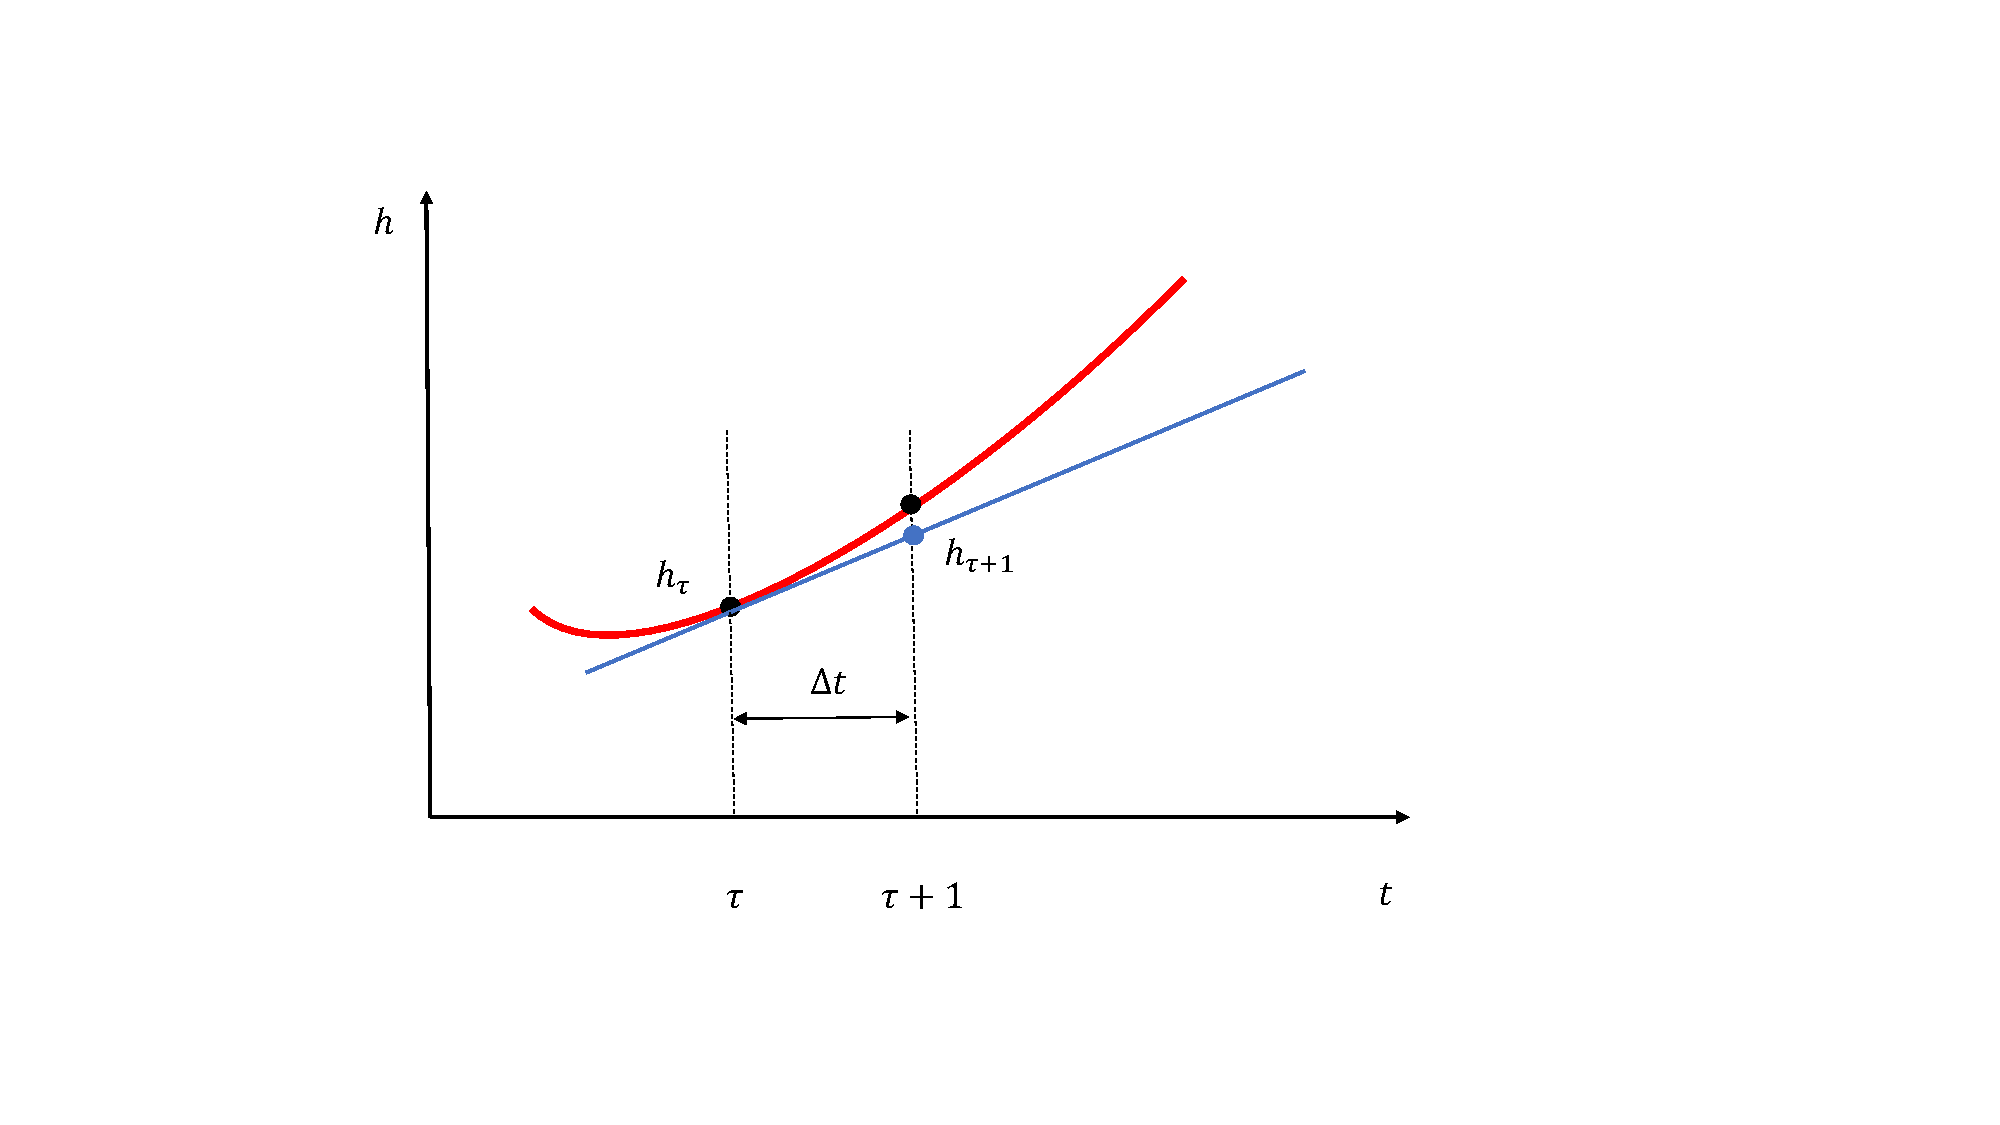
\includegraphics[width=0.6\textwidth]{lecture7-fig1}
\caption{Forward difference method}
\label{fddiagram}
\end{figure}

Note that above the only approximation was done in~\eqref{dhdt1}. We would like to have a way to estimate the error that we made using~\eqref{dhdt1}. Intuitively, one should expect that the error should decrease as we take smaller $\Delta t$, but how fast does the error approaches zero?

To can quantify the performance of a time-stepping scheme, using Taylor series. Recall that any infinitely differentiable function $f(x)$ can be expanded  in a Taylor series as: 
\begin{equation}
f(x_0+a)=f(x_0) + \left.\frac{\partial f}{\partial x}\right|_{x=x_0} a + \left.\frac{\partial^{2}f}{\partial x^{2}}\right|_{x=x_0}\frac{a^{2}}{2!} + O(a^{3}).
\label{TS}
\end{equation}

Applying this to $h$ by taking $x_0=\tau\,\Delta t$ and $a=\Delta t$, we have that
\begin{equation}
h_{\tau+1}=h_{\tau}+\frac{\partial h_{\tau}}{\partial t}\Delta t + O(\Delta t^{2}).
\label{htTS}
\end{equation}

After rearranging terms in \eqref{htTS} and dividing by $\Delta t$,
\begin{equation}
\underbrace{\frac{h_{\tau+1}-h_{\tau}}{\Delta t}}_{(i)}=\underbrace{\frac{\partial h_{\tau}}{\partial t}}_{(ii)} + \underbrace{O(\Delta t)}_{(iii)}.
\label{FOA}
\end{equation}


Since term $(ii)$ the time-derivative of $h$ at $\tau\Delta t$ and term $(i)$ is approximation~\eqref{dhdt1} of this time-derivative, the discrepancy between them expressed in term $(iii)$ is the error. The error for `forward difference' is proportional to $\Delta t$: we say that `forward difference' is a `first-order time-stepping scheme' or is `first order accurate', which means the error decreases linearly with the decrease of the time step. 

Can we do any better? Can we use a different approximation of the time-derivative instead of~\eqref{dhdt1} so that the error is much less?

\subsubsection*{Leapfrog time-stepping}


Instead of using $h_{\tau}$ and $h_{\tau+1}$ to estimate  the derivative, now we use $h_{\tau-1}$ and $h_{\tau+1}$ to do this, leading to 
\begin{equation}
\frac{\partial h_{\tau}}{\partial t}\approx\frac{h_{\tau+1}-h_{\tau-1}}{2\Delta t}.\label{eq7.12}
\end{equation}

This is known as `centred difference' or `leapfrog' method and the schematic diagram is shown in Fig.~\ref{CDdiagram}.
\begin{figure}[h!]
\centering
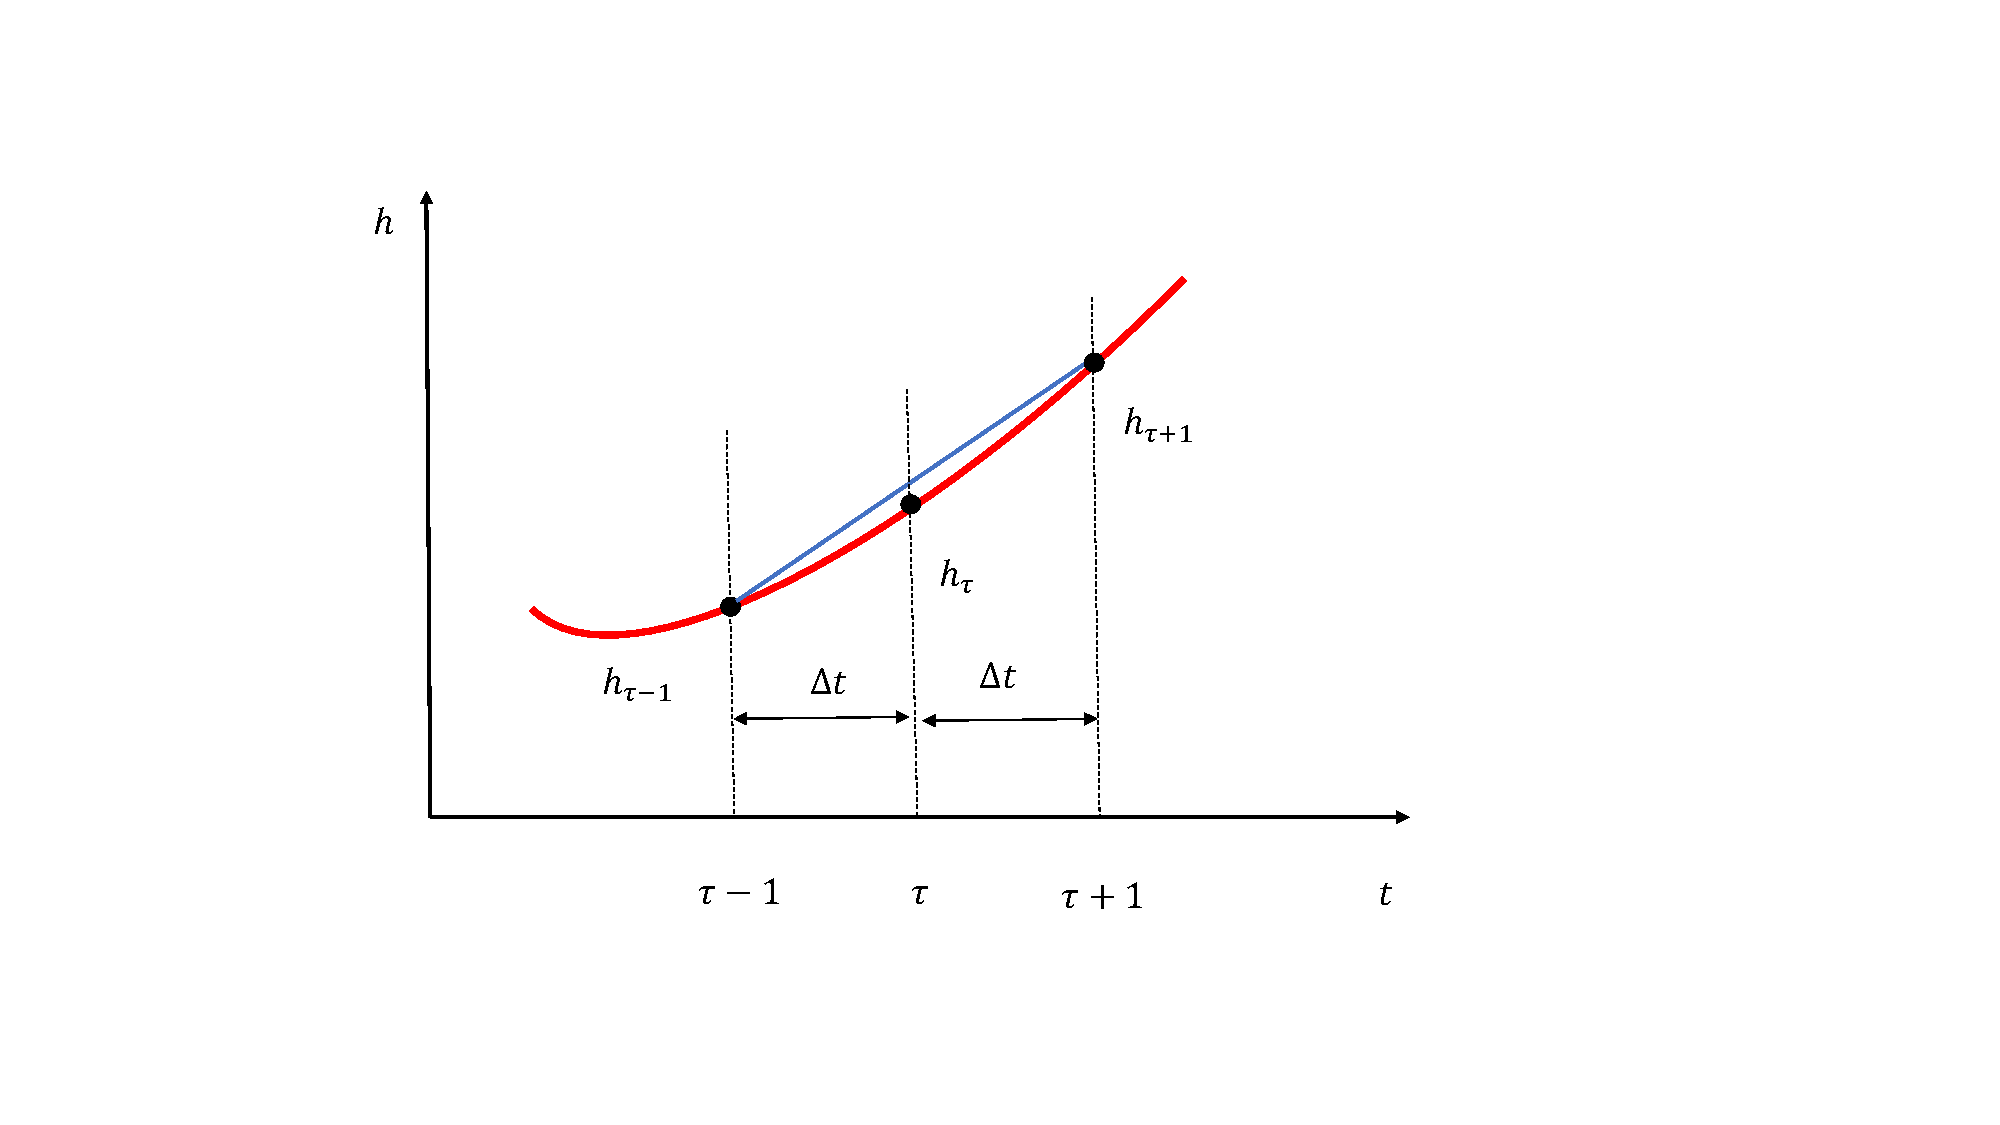
\includegraphics[width=0.5\textwidth]{lecture7-fig2}
\caption{Centred difference method.}
\label{CDdiagram}
\end{figure}

Now, we can repeat the same steps as before to estimate the error we make using~\eqref{eq7.12}. Expand $h_{\tau+1}$ and $h_{\tau-1}$ as a Taylor series:

\begin{align}
	h_{\tau+1}&=h_{\tau}+\frac{\partial h_{\tau}}{\partial t}\Delta t+\frac{\partial^{2}h_{\tau}}{\partial t^{2}}\frac{\Delta t^{2}}{2}+O(\Delta t^{3}),\\
	h_{\tau-1}&=h_{\tau}-\frac{\partial h_{\tau}}{\partial t}\Delta t +\frac{\partial^{2} h_{\tau}}{\partial t^{2}}\frac{\Delta t^2}{2}+O(\Delta t^{3}),
\end{align}

and then subtract them and divide by $2\Delta t$ to form the time-derivative approximation in~\eqref{eq7.12}. We obtain: 
\begin{equation}
	\underbrace{\frac{h_{\tau+1}-h_{\tau-1}}{2\Delta t}}_{(i)}=\underbrace{\frac{\partial h_{\tau}}{\partial t}}_{(ii)}+\underbrace{O(\Delta t^{2})}_{(iii)}.
\label{SOA}
\end{equation}

Similarly as with the forward difference, term $(iii)$ is the error of centred difference method. This time the error is proportional to $(\Delta t)^2$, which is much smaller than $\Delta t$ for small time-steps. Therefore, `centred difference' is second-order accurate and the error declines quadratically as we decrease of the time-step. 

\subsubsection*{A small catch}

The advantage of this `leapfrog' method of time stepping is that it is second order accurate, but it can also induce instability as there are two independent  subsets of the discretised $h_{\tau}$ values that evolve independently without interaction, sometimes leading, possibly, to divergence at some point. Figure~\ref{leapfrog} depicts disconnect between subsets values at $\tau, \tau+2,\tau+4, \dots$ and those at $\tau+1, \tau+3, \dots$: the time grid splits into two subsets (here shown with black and blue) of two independent solutions resulting to numerical instability.

\begin{figure}[h!]
\centering
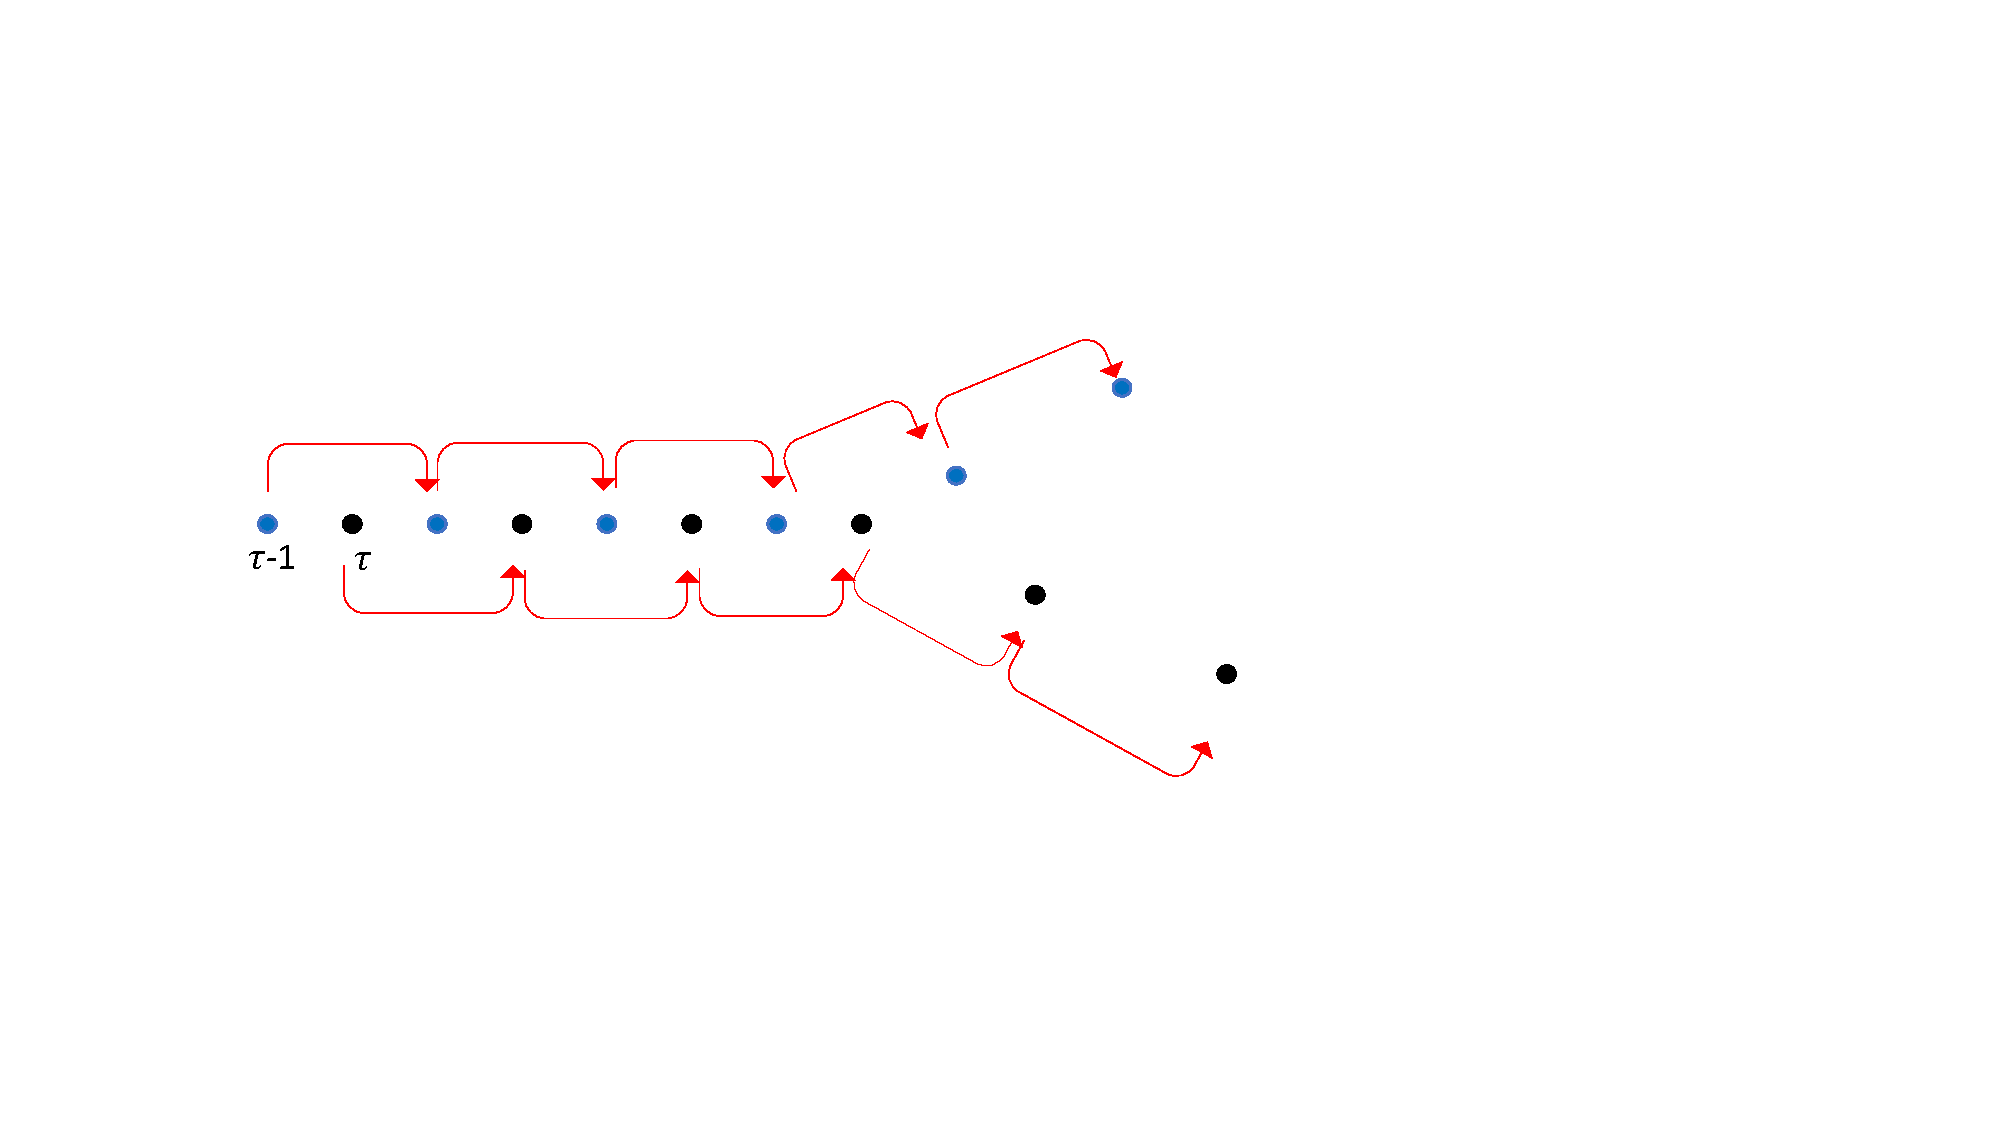
\includegraphics[width=0.5\textwidth]{lecture7-fig3}
\caption{Schematic of numerical instability due to the miscommunication of two different subsets of time-grids when using the leapfrog time stepping scheme.}
\label{leapfrog}
\end{figure}

Therefore, it is necessary to `mix' these two solutions at neighbouring time grid-points to resolve this issue of numerical divergence. To do so, we usually implement a filter on each leapfrog time step. The filter that is  most commonly used is the Robert--Asselin filter:
\begin{equation}
h_{\tau-1}^{R}=h_{\tau-1}+\alpha(h_{\tau}-2h_{\tau-1}+h_{\tau-2}^{R}),
\end{equation}
where $h^{R}$ represents filtered variables. 

We note that implementing Robert-Asselin filter \emph{does} resolve the issue with numerical instability due to the disconnect of the two different time-grid subsets but does come at the expense of the accuracy (the error becomes more than $O(\Delta t)^2$). 

% !TEX root = main.tex

\section{Lecture 8: Barotropic and Baroclinic instabilities}\label{sec:lecture8}
\begin{flushright}\textbf{[by Annie]}\end{flushright}
  
 \begin{itemize}
   \item
   Rossby waves (?)
   \item
   Barotropic instability
   \item
   Baroclinic instability
 \end{itemize}

% !TEX root = main.tex

\section{Lecture 9: Wave--mean flow interactions}\label{sec:lecture9}
\begin{flushright}\textbf{[by Navid]}\end{flushright}
  
 \begin{itemize}
   \item
   Wave--mean flow interactions
 \end{itemize}

% !TEX root = main.tex

\section{Lecture 10: Transformed Eulerian Mean}\label{sec:lecture10}
\begin{flushright}\textbf{[by Navid]}\end{flushright}
  
 \begin{itemize}
   \item
   TEM
 \end{itemize}

% !TEX root = main.tex

\section{Lecture 11: Large-scale ocean circulations}\label{sec:lecture11}
\begin{flushright}\textbf{[by Annie]}\end{flushright}
  
 \begin{itemize}
   \item
   Wind-driven gyres (Stomme/Munk models?)
   \item
   Sverdrup balance
 \end{itemize}

% !TEX root = main.tex

\section{Lecture 12: Title goes here}
\begin{flushright}\textbf{[by ????]}\end{flushright}

\label{sec:lecture12}

% !TEX root = main.tex

\section{Lecture 13: More GVCs: Dia-surface transport}
\begin{flushright}\textbf{[by Eva Cougnon]}\end{flushright}

In this lecture, we develop the concept of dia-surface transport. We can look at it as being a transfer of momentum or tracer across a surface. In previous lectures, we discussed about General Vertical Coordinates (GCVs) and kinematic boundary conditions (lectures~\ref{sec:lecture8} and~\ref{sec:lecture10}), some of what is shown here is based on these two lectures. The goal here is to express the material time derivative operator using GCVs.

\subsection{Flow normal to the surface}
The diagram below illustrates a surface $\sigma$ which is function of space and time, $x, y, z$ and $t$. 
\begin{figure}[h!]
\centering
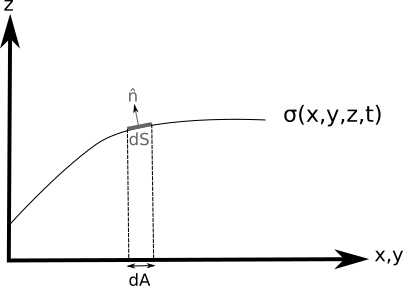
\includegraphics[width=0.4\textwidth]{figures/lecture13_fig1_GVC.png}
\caption{Schematic view of a  dia-surface transport across a surface $\sigma$. The direction normal for a surface element $\mathrm{d}S$ along $\sigma$ is noted $\boldsymbol{\hat{n}}$. The horizontal projection of the surface element $\mathrm{d}S$ is denoted as $\mathrm{d}A = |cos \theta| \mathrm{d}S$, where $\theta$ is the angle between the surface and the horizontal. The vertical stratification should remain non-zero ($\partial_z\sigma\ne0$), the surface element cannot be vertical, so we can relate $\mathrm{d}S$ and $\mathrm{d}A$.
%{\color{red}and should always be different from zero, which means that the surface element cannot be vertical ($\partial \sigma / \partial z \neq 0$). [Navid: The red part here by itself doesn't make sense. The condition $\partial_z\sigma\ne0$ should hold only if we want to relate $dS$ and $dA$.]}
}
\label{schem1}
\end{figure}

By definition, the flux of matter crossing the surface element in the direction normal is equal to:
\begin{equation}
\centering
\text{flux  in  direction } \hat{\boldsymbol{n}} = \boldsymbol{v} \cdot \hat{\boldsymbol{n}},
\label{normal}
\end{equation}
where $\boldsymbol{v}$ is the vector velocity of the fluid particle and where the surface unit normal is:
\begin{equation}
\centering
\hat{\boldsymbol{n}} = \frac{\boldsymbol{\nabla} \sigma}{|\boldsymbol{\nabla} \sigma|}. \label{eq13.2}
\end{equation}

When we take into account that the $\sigma$ surface may move in time, as it is usually the case, the flux of matter across the surface is:
\begin{equation}
\centering
\text{flux of matter crossing surface} = \hat{\boldsymbol{n}} \cdot (\boldsymbol{v}-\boldsymbol{v}^{(\sigma)}),
\end{equation}
where with $\boldsymbol{v}^{(\sigma)}$ we denote the velocity of the surface $\sigma$. The velocity of a point on the surface element satisfies:
\begin{equation}
\frac{\partial \sigma}{\partial t} + \boldsymbol{v}^{(\sigma)} \cdot \boldsymbol{\nabla} \sigma = 0,
\label{partialtimederiv}
\end{equation}
and the material time derivative being:
\begin{equation}
\frac{\mathrm{D}\sigma}{\mathrm{D}t} = \frac{\partial \sigma}{\partial t} + \boldsymbol{v} \cdot \boldsymbol{\nabla} \sigma,
\label{mattimederiv}
\end{equation}
we can estimate the flux of matter crossing the surface by rearranging equations \eqref{partialtimederiv} and \eqref{mattimederiv}:
\begin{equation}
\frac{\mathrm{D}\sigma}{\mathrm{D}t} = - \boldsymbol{v}^{(\sigma)} \cdot \boldsymbol{\nabla} \sigma + \boldsymbol{v} \cdot \boldsymbol{\nabla} \sigma.
\end{equation}

Using equation \eqref{eq13.2} we get:
\begin{equation}
\frac{\mathrm{D}\sigma}{\mathrm{D}t} = \quad |\boldsymbol{\nabla} \sigma|\hat{\boldsymbol{n}} \cdot (\boldsymbol{v}-\boldsymbol{v}^{(\sigma)}),
\end{equation}
and finally the flux of matter across the surface is:
\begin{equation}
\hat{\boldsymbol{n}} \cdot (\boldsymbol{v}-\boldsymbol{v}^{(\sigma)}) = \frac{1}{|\boldsymbol{\nabla} \sigma|} \underbrace{\frac{\mathrm{D} \sigma}{\mathrm{D}t}}_{\equiv \dot{\sigma}}.
\label{fluxacrosssurf}
\end{equation}
where we introduce shorthand $\dot{\sigma}=\mathrm{D}\sigma/\mathrm{D} t$.

This is the net flux of fluid crossing the GVC surface. If no fluid crosses the surface, then the the material time derivative of the GVC surface, $\mathrm{D}\sigma/\mathrm{D}t$, vanishes and vice versa. This results is important in geophysical fluid mechanics and is seen in oceanography in isopycnal models and subduction calculations.


\subsection{Dia-surface transport and its velocity component}

We can use the area of the surface $\mathrm{d}S$ to normalised the volume flux in equation \eqref{fluxacrosssurf}. $\mathrm{d}S$ is an infinitesimal patch on the surface of constant GVC, $\sigma$, with outward unit normal $\boldsymbol{\hat{n}}$, as presented in Figure~\ref{schem1}. $\mathrm{d}A$ is the horizontal projection of this area. Then, the transport of fluid crossing the surface is
\begin{equation}
\frac{\dot{\sigma}}{|\boldsymbol{\nabla} \sigma|} \mathrm{d}S .
\end{equation}

Following rules of trigonometry introduced in lecture~\ref{sec:lecture8} (``Dynamic and permeable surface'') we can express the area factor,  $\mathrm{d}S/|\boldsymbol{\nabla} \sigma|$, as a function of $\mathrm{d}A$. To do so, we need to assume that the values of $\sigma$ depend monotonically with $z$. In that case we introduce the angle $\theta$ between the surface and the horizontal plane. Therefore, $\mathrm{d}A=|\cos \theta| \; \mathrm{d}S$ and the area factor is:
\begin{align} 
\frac{\mathrm{d}S}{|\boldsymbol{\nabla} \sigma|} & = \frac{\mathrm{d}S}{\sqrt{\big(\frac{\partial \sigma}{\partial x}\big)^2+\big(\frac{\partial \sigma}{\partial y}\big)^2+\big(\frac{\partial \sigma}{\partial z}\big)^2}} \nonumber\\
& = \frac{\mathrm{d}S}{\big|\frac{\partial \sigma}{\partial z}\big| \sqrt{ \left(\tfrac{\partial \sigma/\partial x}{\partial \sigma/\partial z}\right)^2 + \left(\tfrac{\partial \sigma/\partial y}{\partial \sigma/\partial z}\right)^2 +1}} \nonumber\\
& = \frac{\mathrm{d}S}{\big|\frac{\partial \sigma}{\partial z}\big| \sqrt{ \left(\frac{\partial z}{\partial x}\right)^2 + \left(\frac{\partial z}{\partial y}\right)^2 +1}} \nonumber\qquad\text{(but }(\tfrac{\partial z}{\partial x})^2 + (\tfrac{\partial z}{\partial y})^2 = \tan^2\theta\text{)} \\
% }_\text{squared slope of surface = $\tan^2\theta$}
& = \frac{\mathrm{d}S}{\big|\frac{\partial \sigma}{\partial z}\big| \sqrt{1 + \tan^2 \theta}} \nonumber\\
& = \biggr\rvert\frac{\partial z}{\partial \sigma}\biggr\lvert \; |\cos \theta| \; \mathrm{d}S \nonumber\\
& = \underbrace{\biggr\rvert\frac{\partial z}{\partial \sigma}\biggr\lvert}_\text{specific thickness} \; \mathrm{d}A.  \label{eq13.10}
\end{align}

Equation~\eqref{eq13.10} allows us to define the dia-surface velocity component for the GVC coordinate system, $w^{(\dot{\sigma})}$, which corresponds to the volume of fluid passing through the surface per unit horizontal area, per unit time:
\begin{equation}
\begin{aligned}
w^{(\dot{\sigma})} & = \hat{\boldsymbol{n}} \cdot (\boldsymbol{v}-\boldsymbol{v}^{(\sigma)}) \frac{\mathrm{d}S}{\mathrm{d}A} \\
& = \frac{(\text{volume}/\text{time}) \: of fluid through surface}{\text{horizontal area of surface}} \\
& = \frac{\partial z}{\partial \sigma} \dot{\sigma}.
\end{aligned}
\label{VelComp1}
\end{equation}
This is a transport with units of velocity and $\partial z/\partial \sigma$ is the specific thickness. An alternative expression that comes from expanding the material time derivative from equation \eqref{fluxacrosssurf}, $\dot{\sigma} = \mathrm{D}\sigma/\mathrm{D}t = |\boldsymbol{\nabla} \sigma| \boldsymbol{\hat{n}} \cdot (\boldsymbol{v} - \boldsymbol{v}^\sigma)$ is:
\begin{align}
w^{(\dot{\sigma})} & =\frac{\partial z}{\partial \sigma} \dot{\sigma} \nonumber\\
& = \frac{\partial z}{\partial \sigma} \bigg (\frac{\partial \sigma}{\partial t} + \boldsymbol{v} \cdot \boldsymbol{\nabla} \sigma \bigg )
\label{wsigma}
\end{align}
By using the equations described above (equation \ref{wsigma}) and partial derivative operators (see \citet[Chapter 18.3 and 8.2 in][]{Griffies2019} for recall on partial derivative operators), we obtain the following equation:
\begin{equation}
w^{(\dot{\sigma})} = w - \bigg [\!\!\!\!\!\underbrace{\bigg (\frac{\partial}{\partial t}\bigg )_\sigma + \boldsymbol{u} \cdot \boldsymbol{\nabla}_\sigma}_{\substack{\text{horizontal material derivative}\\\text{on a surface of constant $\sigma$}}} \!\!\!\!\!\bigg ]z,
\label{VelComp}
\end{equation}
where $(\partial/\partial t)_\sigma$ is the time derivative along the $\sigma$ surface, and $\boldsymbol{\nabla}_\sigma z$ is the slope of the surface.
%[Navid: $(\boldsymbol{u} \cdot \boldsymbol{\nabla}_\sigma)z$ is not dimensionless as a slope should be. Did you meant to write ``$\boldsymbol{\nabla}_\sigma z$ is the slope''?]}.

Equation~\eqref{VelComp} relates the vertical component of the fluid particle velocity $w$ to the dia-surface velocity component $w^{(\dot{\sigma})}$. Therefore, when the GVC surface is static ($\partial z/\partial t$) the dia-surface velocity component described with equation \eqref{VelComp} becomes:
\begin{equation}
w^{(\dot{\sigma})} = w - \boldsymbol{u} \cdot \boldsymbol{\nabla}_\sigma z, \quad \text{for a static surface}.
\end{equation}
On the other hand, when the GVC the surface is flat, the dia-surface velocity components only represent the flux of fluid moving vertically relative to the motion of the GVC surface. But if the surface is both, flat and static (e.g., a constant geopotential), the dia-surface velocity component becomes the vertical velocity component only:
\begin{equation}
w^{(\dot{\sigma})} = w = \frac{\mathrm{D}z}{\mathrm{D}t}, \quad \text{for a static and flat surface}.
\end{equation}

\subsection{Material time-derivative in GVCs}

With the expression of the dia-surface velocity component for the GVC system, $w^{(\dot{\sigma})}$, equation~\eqref{VelComp1}, we can express the material time-derivative in three different ways which turn out to be useful in GVCs:
\begin{equation}
\begin{aligned}
\left(\frac{\mathrm{D}}{\mathrm{D}t}\right)_z & = \bigg (\frac{\partial}{\partial t} \bigg )_z + \underbrace{\boldsymbol{u} \cdot \boldsymbol{\nabla}_z}_{\substack{\text{horizontal}\\\text{gradient}}} \;\; +\!\!\!\! \underbrace{w\frac{\partial}{\partial z}}_{\substack{\text{gradient of}\\\text{vertical velocity}}} \\
\substack{\text{changing from Cartesian}\\\text{coordinates to GVCs:}}& =  \bigg (\frac{\partial}{\partial t} \bigg )_\sigma + \boldsymbol{u} \cdot \boldsymbol{\nabla}_\sigma + \underbrace{w^{(\dot{\sigma})}\frac{\partial}{\partial z}}_{\substack{\text{non-zero  transport}\\\text{across the surface}}} \\
& =  \bigg (\frac{\partial}{\partial t} \bigg )_\sigma + \boldsymbol{u} \cdot \boldsymbol{\nabla}_\sigma + \dot{\sigma}\frac{\partial}{\partial \sigma}.
\end{aligned}
\end{equation}
The relationship between  the two vertical coordinate partial derivative comes from the chain rule:
\begin{equation}
\frac{\partial}{\partial \sigma} = \frac{\partial z}{\partial \sigma} \frac{\partial}{\partial z}.
\end{equation}

\subsection{Velocity vector and fluid particle trajectories}

The velocity vector in Cartesian coordinates is:
\begin{equation}
\boldsymbol{v} = \boldsymbol{\hat{x}}u + \boldsymbol{\hat{y}}v + \boldsymbol{\hat{z}}w,
\end{equation}
and using $w$ from equation~\eqref{VelComp} we get:
\begin{equation}
\boldsymbol{v} =  \boldsymbol{\hat{x}}u + \boldsymbol{\hat{y}}v + \boldsymbol{\hat{z}} \bigg [w^{(\dot{\sigma})} + \bigg (\frac{\partial z}{\partial t} \bigg )_\sigma + \boldsymbol{u} \cdot\boldsymbol{\nabla}_\sigma z \bigg].
\end{equation}
By re-arranging and combining the $u$ terms we get:
\begin{align}
\boldsymbol{v} &=  u\underbrace{\bigg [\boldsymbol{\hat{x}} + \boldsymbol{\hat{z}}  \bigg (\!\overbrace{\frac{\partial z}{\partial x}}^{\substack{\text{slope}\\\text{term}}} \! \bigg )_\sigma \bigg]}_{=\boldsymbol{e}_{\bar{1}}} 
+ v  \underbrace{\bigg [\boldsymbol{\hat{y}} + \boldsymbol{\hat{z}}  \bigg (\!\overbrace{\frac{\partial z}{\partial y}}^{\substack{\text{slope}\\\text{term}}} \!\bigg )_\sigma \bigg]}_{=\boldsymbol{e}_{\bar{2}}} 
+ \bigg [ \bigg (\frac{\partial z}{\partial t}\bigg )_\sigma + w^{(\dot{\sigma})} \bigg]\boldsymbol{\hat{z}} \nonumber\\
&=  u\,\boldsymbol{e}_{\bar{1}} + v\,\boldsymbol{e}_{\bar{2}} + \bigg [ \bigg (\frac{\partial z}{\partial t}\bigg )_\sigma + w^{(\dot{\sigma})} \bigg]\boldsymbol{\hat{z}}.
\label{vel}
\end{align} 

Equation~\eqref{vel} gives the flow components in the GVC system. We notice that the horizontal components remain the same as in Cartesian coordinates but the third components changes.

To elucidate these velocity expressions, below are three examples where we ignore the $y$-direction and consider the particle moving only in the $x$- and $z$-directions. This implies that the second term in equation \eqref{vel} is ignored.

\subsubsection*{Example A -- Steady and material $\sigma$-surface in $x$-direction} 

As we assume the surface to be steady, $\partial \sigma/ \partial t = 0$, and the material surface implies $\mathrm{D}\sigma/\mathrm{D}t = \dot{\sigma} = 0$. The latter implies $w^{(\dot{\sigma})} = 0$ from equation \eqref{wsigma}, and the fluid does not cross the surface. With these two conditions, the third term in equation \eqref{vel} goes also to zero. The velocity vector is:
\begin{equation}
\boldsymbol{v} =  u\bigg [\boldsymbol{\hat{x}} + \boldsymbol{\hat{z}}  \bigg (\frac{\partial z}{\partial x} \bigg )_\sigma \bigg] ,
\end{equation}
as illustrated by the Figure~\ref{exA}.

\begin{figure}[h!]
	\centering
	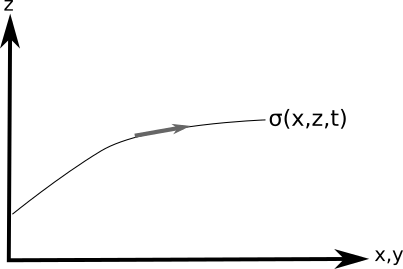
\includegraphics[width=0.4\textwidth]{figures/lecture13_exampleA.png}
	\caption{Schematic view of the steady and material $\sigma$-surface case, where the flow is along the surface. The grey vector shows the vector of the fluid particle velocity between time $t$ and $t+\delta t$.}
	\label{exA}
\end{figure}

\subsubsection*{Example B -- Non-steady and material $\sigma$-surface in $x$-direction} 


In this case, the material $\sigma$-surface ($\mathrm{D}\sigma/\mathrm{D}t = \dot{\sigma} = 0$) moves in time $\partial \sigma / \partial t \neq 0$. Therefore, the velocity vector becomes:
\begin{equation}
\boldsymbol{v} = \underbrace{u\bigg [\boldsymbol{\hat{x}} + \boldsymbol{\hat{z}}  \bigg (\frac{\partial z}{\partial x} \bigg )_\sigma \bigg]}_\text{motion along the surface}
	+ \underbrace{\bigg [ \bigg (\frac{\partial z}{\partial t}\bigg )_\sigma \bigg]\boldsymbol{\hat{z}}}_{\substack{\text{takes particle}\\\text{to the new $\sigma$-surface}}} ,
\end{equation}
as illustrated by the Figure~\ref{exB}.


\begin{figure}[h!]
	\centering
	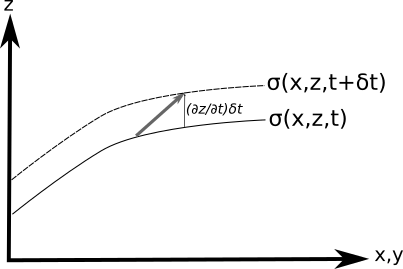
\includegraphics[width=0.4\textwidth]{figures/lecture13_exampleB.png} 
	\caption{Schematic view of the non-steady and material $\sigma$-surface case, where the fluid particle must move vertically relative to the static $\sigma$-surface. The grey vector shows the vector of the fluid particle velocity between time $t$ and $t+\delta t$.}
	\label{exB}
\end{figure}


\subsubsection*{Example C -- Non-steady and non-material $\sigma$-surface in $x$-direction} 

In this case, $\mathrm{D}\sigma/\mathrm{D}t = \dot{\sigma} \neq 0$ and $\partial \sigma/ \partial t \neq 0$. The third term in equation \eqref{vel}, including the dia-surface velocity ($w^{(\dot{\sigma})}$), cannot be neglected. $w^{(\dot{\sigma})}$ is the transport across the surface, which is not necessarily solely horizontal or vertical. Therefore, the velocity vector is:
\begin{equation}
\boldsymbol{v} = u\bigg [\boldsymbol{\hat{x}} + \boldsymbol{\hat{z}}  \bigg (\frac{\partial z}{\partial x} \bigg )_\sigma \bigg]
+ \bigg [ \bigg (\frac{\partial z}{\partial t}\bigg )_\sigma + \underbrace{w^{(\dot{\sigma})}}_{\substack{\text{dia-surface}\\\text{velocity}}} \bigg]\boldsymbol{\hat{z}} ,
\end{equation}
as illustrated by the Figure~\ref{exC}.

\begin{figure}[h!]
	\centering
	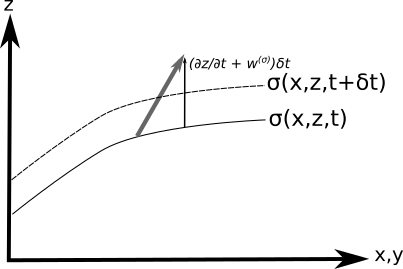
\includegraphics[width=0.4\textwidth]{figures/lecture13_exampleC.png}
	\caption{Schematic view of the non-steady and non-material $\sigma$-surface case, where the fluid particle must move vertically relative to the static $\sigma$-surface and cross the $\sigma$-surface. The grey vector shows the vector of the fluid particle velocity between time $t$ and $t+\delta t$, which departed from the $\sigma$-surface due to the nonzero dia-surface velocity component.}
	\label{exC}
\end{figure}

For more details, also read \citep[Chapter 18.3-18.6 in][]{Griffies2019}.
% !TEX root = main.tex

\section{Lecture 14: Title goes here}
\begin{flushright}\textbf{[by ????]}\end{flushright}



% !TEX root = main.tex

\section{Lecture 15:  Arbitrary Lagrangian--Eulerian scheme}
\begin{flushright}\textbf{[by Christelle Auguste]}\end{flushright}

{\color{red} Navid: I'm working on these notes.}

The Arbitrary Lagrangian--Eulerian (ALE) method combines the best features of Lagrangian and Eulerian representations. In Lagrangian simulations the mesh moves with the local velocity, in Eulerian  simulations the mesh is fixed in space and the fluid moves from one cell to another. The initial representation of the ALE method was described by \citet{1974JCoPh..14..227H}. There are two general methods of ALE in ocean models: quasi-Eulerian and quasi-Lagrangian algorithm (used by MOM6). This lecture focuses on the latter.

The added features of the ALE method provide the opportunity to increase the model time step (removal of the vertical Courant--Friedrichs--Lewy). The stability criterion known as Courant--Friedrichs--Lewy condition or CFL condition is:
\begin {align}
\mathrm{CFL}&=\Delta t <\frac{\Delta x}{2c}.
\end{align}
with the CFL number equal to :
\begin{equation}
C \equiv \frac{u \Delta t}{\Delta x}.
\end{equation}
The Courant number is a measure of how much information traverses $u$ a computational grid cell $\Delta x$ in a given time-step $\Delta t$.
The time step must be less than a certain time in many explicit time marching computer simulations, otherwise the simulation will produce incorrect results. CFL condition it is necessary to define correctly the time step simulation. The Courant number must be equal or smaller than 1, otherwise, the numerical viscosity would be negative.

{\color{red}[Navid: 1. Please punctuate equations.]}\\
{\color{red}[Navid: 2. The CFL is a non-dimensional number $u dt/dx$ and this number should be less than 1 or 0.5 for the simulation to be stable. Can you 1) fix your definition above and 2) provide a bit more details for what CFL is and why it should be less than one? (I mean 1-2 sentences...). If you need help let me know.]}\\

Consider
\begin{equation}
    \frac{\partial p}{\partial z} =- g \rho (Z, \delta^n, \sigma^n).
\end{equation}
with $n = \text{time level}$.

Now consider the Boussinesq hydrostatic equations for thickness:
 \begin{equation}
     \frac{\partial h}{\partial t} + \boldsymbol{\nabla}_\sigma \cdot(h \boldsymbol{U})+\Delta_\sigma (w^{\dot{\sigma }})=0.
 \end{equation}
 with $w^{\dot{\sigma }}$ equal to the Dia-surface velocity component.
 \begin{figure}[h!]
  \centering
  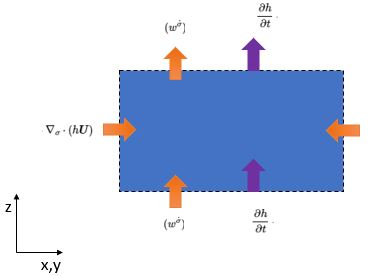
\includegraphics[width=3in]{lecture15_thicknessequation}
    \caption{Mapping of Thickness equation }
  \end{figure}

 \begin{equation}
     \frac{h^{n+1}-h^n}{\Delta t}= -\boldsymbol{\nabla}_\sigma(h\boldsymbol{U})- \Delta_\sigma (w^{\dot{\sigma }}).
 \end{equation}

 where ${\Delta_\sigma (w^{\dot{\sigma }}})$ is negligible, which gives:
  \begin{equation}
     h^\dagger=h^n-\Delta t \boldsymbol{\nabla}_\sigma(h\boldsymbol{U}^n)\label{L15:Regrid}.
 \end{equation}
 with $h^\dagger$ an incomplete version of $h^{n+1}$, the one we are looking for.
 
 We use the same process for $\boldsymbol{U}$ and we obtain:
 \begin{equation}
     \boldsymbol{U}^\dagger=\boldsymbol{U}^n-\Delta t (...).
 \end{equation}
 \\$h^\dagger$ and $\boldsymbol{U}^\dagger$ are  solutions to the shallow water equations.
 
 Concretely in the model we discretised with Lagrangian form at the beginning of the simulation, the second step in the algorithm is to regrid then to remap. 
 \\On Figure 15.1 are represented this steps used to time step the fluid state. The step regrid acts to reinitialize the vertical coordinate by locating the new vertical grid, the corresponding equation is Eq.~\eqref{L15:Regrid}: the new thickness is prescribed by the new grid. In this step the advection is no longer linked to CFL. The step remap acts to remap all variables from the old grid onto the new grid, and the corresponding equation for remap tracer is:
  \begin{equation}
     h^\dagger C^\dagger=h^nC^n+\Delta t \boldsymbol{\nabla}_\sigma(\boldsymbol{U}^nC^n)\label{L15:Remap}.
 \end{equation}
 %is it right for the last term?? was not written by Andy....
 
  \begin{figure}[h!]
  \centering
  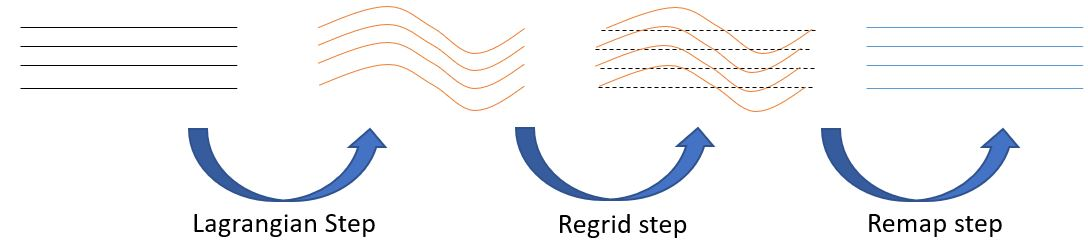
\includegraphics[width=5in]{figures/lecture15_stepsale.JPG}
  \caption{Steps for ALE algorithm. (Figure modified from \citet{Griffies2019}.) {\color{red}[Navid: Christelle, can you remove the red spell-checking underlines from the figure labels?] // Done}}
  \end{figure}

Example with internal waves, consider $\eta_k ^0$ 

when Z goes to infinity, when remapping instead of going back to the initial state we have:
 \begin{equation}
  \eta_{k}^{n+1} = \frac{(\eta_{k}^\dagger - \eta_{k}^0)\Delta t}{\tau}.
 \end{equation}
 with $\tau$ the time scale
 \\If the time step is fast, less than a day this step stay the same, and over a long term period come back to zero: the long term evolution of the ocean is not Lagrangian.
 
 
  Case of Adaptive grid:
  \begin{equation}
     \frac{\partial \eta_k}{\partial t} =- \boldsymbol{\nabla}_\sigma(\alpha_\sigma\frac{k\boldsymbol{\nabla}_\sigma \rho}{\sqrt{(\partial{z} \rho)^2+(\boldsymbol{\nabla}_\sigma \rho)^2}}+\alpha_\sigma K\boldsymbol{\nabla}_\sigma \eta_k) .
 \end{equation}
 %% don't know how to explain this equation!
  \begin{figure}[h!]
  \centering
  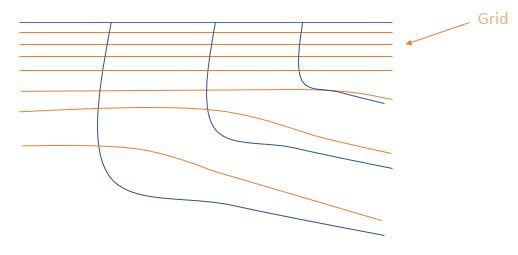
\includegraphics[width=5in]{figures/lecture15_adaptivegrid.JPG}
    \caption{Schematic adaptive grid.}
    \label{fig:lecture15_adaptivegrid}
    \end{figure}
  In this case the grid is following the isopycnal.
  
 In ocean models, mixing has two components : physical and numerical.The physical comes from advection by unresolved turbulence (diffusivity), and numerical from errors in the discretisation to solve the governing equations \citep{GIBSON201745}.Numerical mixing is also called spurious mixing, and we aim to minimise this term. ALE method can reduce spurious mixing by remapping to continuous isopycnal coordinates (Fig. \ref{fig:lecture15_adaptivegrid}).
 

% !TEX root = main.tex

\section{Lecture 16: Form stress}
\begin{flushright}\textbf{[by Luwei Yang]}\end{flushright}

%The following relationships are commonly used in the derivation in this lecture and therefore are listed at the beginning. 

In this lecture, we derive the expression of form stress {\color{red}in the density coordinates}.

{\color{red}[Navid: this may read to someone that form-stress is an `artefact' of the particular coordinate system while, in fact, it is much more general than that... Do you agree?]}

We assume that the ocean can be divided by $N-1$ interfaces into $N$ density layers (see figure~\ref{fig:lecture16_form_stress_schematic}). 

\begin{figure}[!ht]
    \centering
    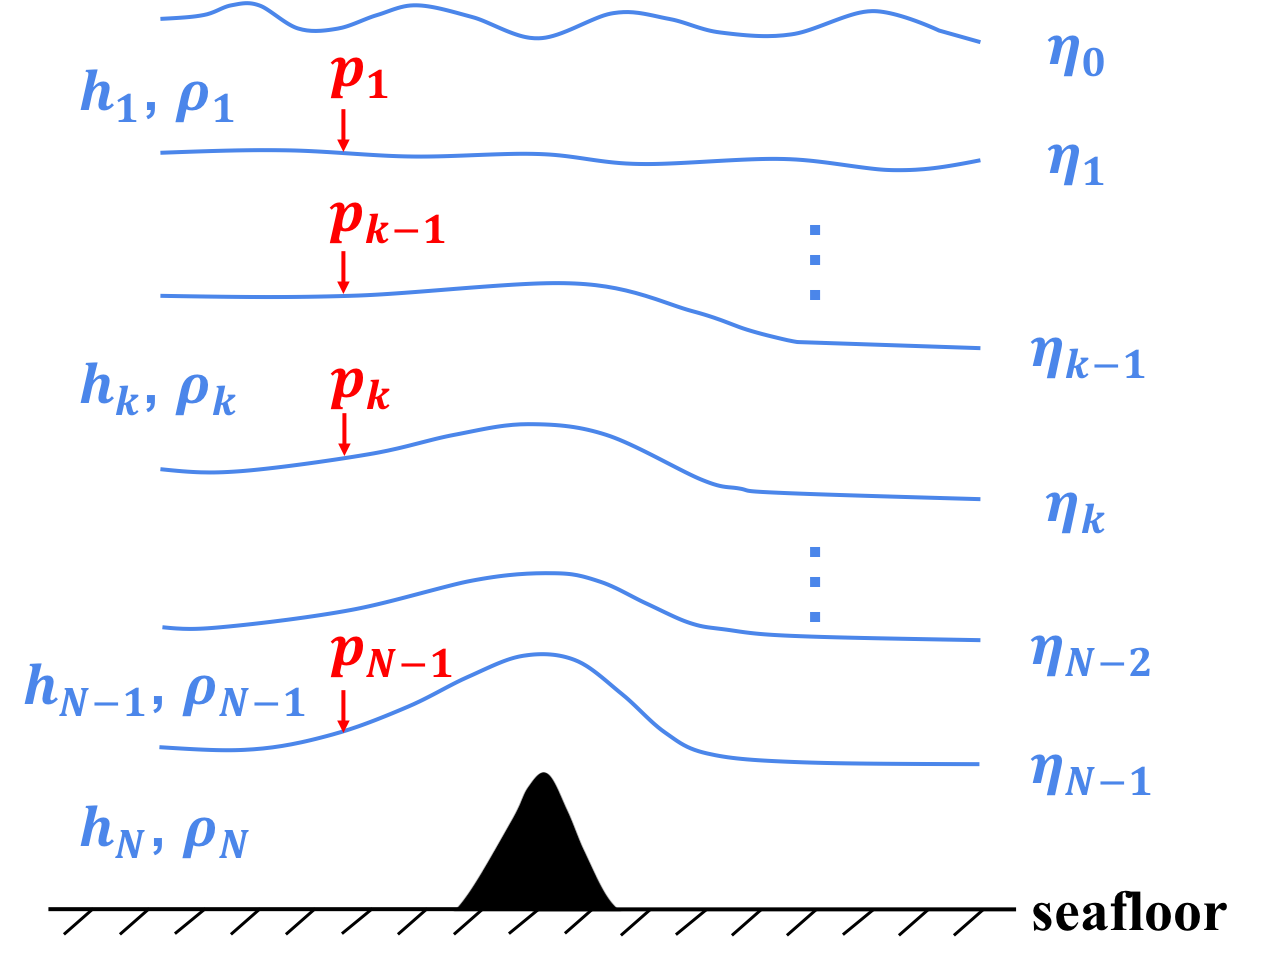
\includegraphics[width=0.6\textwidth]{lecture16_fig1}
    \caption{A schematic of density layers in the ocean.}
    \label{fig:lecture16_form_stress_schematic}
\end{figure}

We define the $k$-th layer ($k = 1, 2, \dots, N$) as the layer between the $(k-1)$-th and $k$-th interface. Under this definition, layer 1 is bounded by sea surface and the first interface, whereas the $N$-th  layer is bounded by the $(N-1)$-th interface and seafloor. The density of layer~$k$ is $\rho_{k}$. The height of the $k$-th fluid interface is denoted as $\eta_k$; $\eta_0$ is the sea surface elevation. The thickness of layer~$k$ is $h_{k}$ and satisfies
\begin{equation}
    h_{k} = \eta_{k-1} - \eta_{k}.
    \label{eq: thickness}
\end{equation}

{\color{red}[Navid: I simplified the above a bit... E.g., you had $k=1,\dots,N$ written 3-4 times...]}

The pressure felt by the $k$-th interface is $p_{k}$; the net pressure of layer $k$ is written as
\begin{equation}
    p_{k} - p_{k-1} = \rho_{k}gh_{k}.
    \label{eq: net_pressure}
\end{equation}
 
{\color{red}[Navid: OK, up to here you were just introducing definition. I think now we need 1-2 sentences of what's the plan... If you simply press on by defining $M$ and then do these algebraic acrobatics leaves one wondering where are all this is heading.... ]}
 
The Montgomery potential \textit{M} is defined as
\begin{equation}
    M = \frac{p + \rho gz}{\rho_{0}},
    \label{eq: M_def}
\end{equation}
where $p$ is pressure, $\rho$ density, $g$ the gravitational acceleration, and $\rho_{0}$ the reference density. 
The Montgomery for layer $k$ is therefore 
\begin{equation}
    M_{k} = \frac{1}{\rho_{1}}(p_{k} + \rho_{k}g\eta_{k}),
    \label{eq: M_k}
\end{equation}
{\color{red}where we use the density of first layer ($\rho_{1}$) as reference density. [Navid: do we need to use $\rho_1$ as ref density and create complications? I think this adds to the confusion. Can't we just leave it $\rho_0$? Actually the ref density should be the mean density of the fluid...]}
We also define $G_{k}$ as
\begin{equation}
    G_{k} = \frac{g\rho_{k}}{\rho_{1}}.
    \label{eq: G_k_def}
\end{equation}
The Montgomery of layer $k$ ($M_{k}$) can be rewritten as
\begin{equation}
    M_{k} = \frac{1}{\rho_{1}}\frac{1}{2}(p_{k} + p_{k-1}) + 
            \frac{1}{\rho_{1}}\frac{1}{2}(p_{k} - p_{k-1}) + G_{k}\eta_{k}.
    \label{eq: M_k_expaned}
\end{equation}
We denote the first term on the right hand side of Eq. \eqref{eq: M_k_expaned} as $P_{k}$,
\begin{equation}
    P_{k} = \frac{1}{2\rho_{1}}(p_{k} + p_{k-1}).
    \label{eq: P_k_def}
\end{equation}
The second term on the right hand side of Eq. \eqref{eq: M_k_expaned} can be rewritten by using Eq. \eqref{eq: net_pressure}, Eq. \eqref{eq: M_def}, and Eq. \eqref{eq: thickness}. Following Eq. \eqref{eq: M_k_expaned}, we then have
\begin{align}
\begin{split}
    M_{k} & = P_{k} + \frac{1}{\rho_{1}}\frac{1}{2}(p_{k} - p_{k-1}) + G_{k}\eta_{k} \\
          & = P_{k} + \frac{1}{\rho_{1}}\frac{1}{2}\rho_{k}gh_{k} + G_{k}\eta_{k} \\
          & = P_{k} + \frac{1}{2}G_{k}h_{k} + G_{k}\eta_{k} \\
          & = P_{k} + \frac{1}{2}G_{k}(\eta_{k-1} - \eta_{k}) + G_{k}\eta_{k} \\
          & = P_{k} + \frac{1}{2}G_{k}\eta_{k-1} + \frac{1}{2}G_{k}\eta_{k}
\end{split}
\label{eq: M_k_final}
\end{align}

We have derived the momentum equation ($x$-direction) for layer $k$ in Lecture~\ref{sec:lecture12}, {\color{red}[Navid: stress here that (16.9) is without any frictional terms!]}
\begin{equation}
    \frac{\partial h_{k}u_{k}}{\partial t} + \frac{\partial h_{k}u_{k}u_{k} }{\partial x} + \frac{\partial h_{k}u_{k}v_{k} }{\partial y} - f h_{k} v_{k} = - h_{k}\boldsymbol{\nabla} M_{k},
\end{equation}
or its vector form (\textcolor{red}{I don't understand how to get the vector form or what I have here is correct or not}),

{\color{red}[Navid: What do you mean? You don't understand how eqs. (16.10) and (16.9) are related?]}

\begin{equation}
    \frac{\partial h_{k}\boldsymbol{u}_{k}}{\partial t} + \boldsymbol{\nabla} ( h_{k} \boldsymbol{u}_{k} \boldsymbol{u}_{k}) + f \boldsymbol{z} \times h_{k} \boldsymbol{u}_{k} = - h_{k}\boldsymbol{\nabla} M_{k},
    \label{eq: momentum_density_coord}
\end{equation}
which shows that it is key to get an expression of $h_{k}\boldsymbol{\nabla} M_{k}$ for the derivation of form stress.
Let's expand $h_{k}\boldsymbol{\nabla} M_{k}$ using Eq. \eqref{eq: M_k_final},
\begin{align}
    \begin{split}
        h_{k}\boldsymbol{\nabla} M_{k} & = h_{k} \boldsymbol{\nabla} (P_{k} + \frac{1}{2}G_{k}\eta_{k-1} + \frac{1}{2}G_{k}\eta_{k})\\
        & = h_{k}\boldsymbol{\nabla} P_{k} + \frac{1}{2}h_{k}G_{k}\boldsymbol{\nabla} \eta_{k-1} + \frac{1}{2}h_{k}G_{k}\boldsymbol{\nabla} \eta_{k} \\
        & = \boldsymbol{\nabla} (h_{k}P_{k}) - P_{k} \boldsymbol{\nabla} h_{k} + \frac{1}{2}h_{k}G_{k} \boldsymbol{\nabla} (\eta_{k-1} + \eta_{k}) 
    \end{split}
    \label{eq: h_grad_M}
\end{align} 
Using Eq. \eqref{eq: P_k_def} and Eq. \eqref{eq: thickness}, we can rewrite the second term on the right hand side of Eq. \eqref{eq: h_grad_M} as 
$$P_{k} \boldsymbol{\nabla} h_{k} = \frac{1}{2\rho_{1}}(p_{k} + p_{k-1}) \boldsymbol{\nabla} (\eta_{k-1} - \eta_{k}). $$
Using Eq. \eqref{eq: net_pressure} and Eq. \eqref{eq: G_k_def}, we can rewrite the third term on the right hand side of Eq. \eqref{eq: h_grad_M} as
$$\frac{1}{2}h_{k}G_{k} \boldsymbol{\nabla} (\eta_{k-1} + \eta_{k}) = \frac{1}{2\rho_{1}}(p_{k} - p_{k-1}) \boldsymbol{\nabla} (\eta_{k-1} + \eta_{k}). $$
Following Eq. \eqref{eq: h_grad_M}, we have
\begin{align}
    \begin{split}
        h_{k}\boldsymbol{\nabla} M_{k} & = \boldsymbol{\nabla} (h_{k}P_{k}) - 
        \frac{1}{2\rho_{1}}(p_{k} + p_{k-1}) \boldsymbol{\nabla} (\eta_{k-1} - \eta_{k}) + 
        \frac{1}{2\rho_{1}}(p_{k} - p_{k-1}) \boldsymbol{\nabla} (\eta_{k-1} + \eta_{k}) \\ 
        & = \boldsymbol{\nabla} (h_{k}P_{k}) + 
        \frac{p_{k}}{2\rho_{1}} (\cancel{-\boldsymbol{\nabla} \eta_{k-1}} + \boldsymbol{\nabla} \eta_{k} \cancel{+ \boldsymbol{\nabla} \eta_{k-1}}  + \boldsymbol{\nabla} \eta_{k} ) + 
        \frac{p_{k-1}}{2\rho_{1}} (- \boldsymbol{\nabla} \eta_{k-1} \cancel{+\boldsymbol{\nabla} \eta_{k}} - \boldsymbol{\nabla} \eta_{k-1}  \cancel{- \boldsymbol{\nabla} \eta_{k}}) \\
        & = \boldsymbol{\nabla} (h_{k}P_{k}) + \frac{p_{k}}{\rho_{1}} \boldsymbol{\nabla} \eta_{k} - \frac{p_{k-1}}{\rho_{1}} \boldsymbol{\nabla} \eta_{k-1}.
    \end{split}
    \label{eq: h_grad_M_final}
\end{align} 
Substitute Eq. \eqref{eq: h_grad_M_final} into Eq. \eqref{eq: momentum_density_coord}, we have
\begin{equation}
    \frac{\partial h_{k}\boldsymbol{u}_{k}}{\partial t} + \boldsymbol{\nabla} ( h_{k} \boldsymbol{u}_{k} \boldsymbol{u}_{k} + h_{k} P_{k} ) + f \boldsymbol{z} \times h_{k} \boldsymbol{u}_{k} = - \frac{p_{k}}{\rho_{1}} \boldsymbol{\nabla} \eta_{k} + \frac{p_{k-1}}{\rho_{1}} \boldsymbol{\nabla} \eta_{k-1}.
    \label{eq: momentum_updated}
\end{equation}

{\color{red}[Navid: I think here the reader deserves a break. Let's add 1-2 sentences discussing eq.~\eqref{eq: momentum_updated} before heading below to an application. For example one can discuss: 1) Why was it important to do all these acrobatics so that we pulled the $h_k P_k$ term inside the divergence on the LHS? 2) What do the terms on the RHS are? Say that these terms induce momentum exchange between layers in the absence of any frictional stress! This way you can connect with the remark made regarding eq. (16.9). In my opinion that's the `amazing' thing with the form stress terms... (and also I think that's what most people have trouble digesting). ]}




For statistically steady state, the zonal average (e.g., around the Southern Ocean) of x-component of Eq. \eqref{eq: momentum_updated} yields 
\begin{equation}
    - f \overline{ h_{k}v_{k} } = \overline{ \frac{p_{k-1}}{\rho_{1}} \frac{ \partial \eta_{k-1} }{ \partial x } } - \overline{ \frac{p_{k}}{\rho_{1}} \frac{ \partial \eta_{k} }{ \partial x } },
    \label{eq: momentum_zonal_ave}
\end{equation}
Integrate Eq. \eqref{eq: momentum_zonal_ave} throughout the water column, assuming that surface buoyancy fluxes allow the water mass transformation to happen at a rate to ensure the net volume exchange across this zonal band is zero, we then obtain
\begin{equation}
    0 = \cancel{ \overline{ \frac{p_{0}}{\rho_{1}} \frac{ \partial \eta_{0} }{ \partial x } } }  - \overline {\frac{p_{N}}{\rho_{1}} \frac{ \partial \eta_{N} }{ \partial x }} + \overline{\tau_{wind}}, 
\end{equation}
where $\tau_{wind}$ is the surface wind stress, which is from the vertical integration of vertical viscous term (not shown in equations). We can rewrite the equation above as
\begin{equation}
    \overline{\tau_{wind}} = \overline{\frac{p_{N}}{\rho_{1}} \frac{ \partial \eta_{N} }{ \partial x }},
    \label{eq: momentum_zonal_ave_final}
\end{equation}
where $p_{N}$ is bottom pressure and $\eta_{N}$ the depth of the ocean. The right hand side of Eq. \eqref{eq: momentum_zonal_ave_final} is essentially the pressure difference across topography, a.k.a topographic form stress. Eq. \eqref{eq: momentum_zonal_ave_final} shows the zonally averaged momentum balance: (in the real ocean, 95\% of the) surface wind stress is balanced by topographic form stress. 
Note we ignore the contribution from bottom frictional drag to momentum balance as it is much smaller than wind stress or topographic form stress.

\textcolor{gray}{exercise will be written soon...}
% !TEX root = main.tex

\section{Lecture 17: Title goes here}
\begin{flushright}\textbf{[by ????]}\end{flushright}



% !TEX root = main.tex

\section{Lecture 18: Title goes here}
\begin{flushright}\textbf{[by ????]}\end{flushright}

% please write the title when you start writing the notes
% this way I know by glancing the table of contents where to look
% cheers, Navid


% !TEX root = main.tex

\section{Lecture 19: Friction \& Stress in models}
\begin{flushright}\textbf{[by Craig Stewart and David Gwyther]}\end{flushright}

Intro paragraph
- need to treat frictional dissipation in models\\
- that term in NS that we kept ignoring.\\
- split into internal frictional dissipation (i.e. straight from lectures)\\
- and frictional dissipation at the vertical boundaries (application from ice/ocean BL theory that we write from scratch)\\


Fluid elements are subject to two general kinds of force; body forces, which act through the medium in proportion to mass, and contact forces, which are transmitted between adjacent regions of fluid. Body forces include gravity, electromagnetic forces, and the apparent Coriolis force. Contact forces, generated by the interaction of fluid elements with their neighbours, are represented by the second order stress tensor $\boldsymbol{T}$. These interactions between adjacent fluid elements provide the means to move momentum between regions of the fluid, and through molecular viscosity, to dissipate kinetic energy into heat, and are the essential difference between particle and continuum mechanics.  % Griffies Sec 26.1

Newton's second law, applied to a control volume $\partial V$ of fluid with density $\rho$, and baricentric velocity $v$, provides the Eularian conservation of momentum equation,\\
\begin{equation}
    \rho\frac{D\boldsymbol{v}}{Dt} = \rho\boldsymbol{f} +  \boldsymbol{\nabla}\cdot\boldsymbol{T}.
    \label{L19:GeneralFormMomentum}
\end{equation}
This simply states that the material acceleration of the fluid times its density, is equal to the sum of forces acting on the element, including the body force $\rho \boldsymbol{f}$ and the contact force $\boldsymbol{\nabla}\cdot\boldsymbol{T}$. Although the contact force is the integral of $\boldsymbol{T}$ over the fluid element surface, Gauss's law allows us to write this as the volume integral of $\boldsymbol{\nabla}\cdot\boldsymbol{T}$ over the fluid volume $\partial V$.

In three dimensional Cartesian space the stress tensor $\boldsymbol{T_{ij}}$ has 9 elements that describe the three orthogonal stresses acting on each of three planes orthogonal to the Cartesian basis vectors. 
\begin{equation}
T = 
\begin{bmatrix}
T_{xx}&T_{xy}&T_{xz}\\
T_{yx}&T_{yy}&T_{yz}\\
T_{zx}&T_{zy}&T_{zz}.\\
\end{bmatrix}
\end{equation}
Here the first index describes the direction of the stress component, and the second index describes the face normal direction.\\
%These describe the component of stress in the $i_{th}$ dimension acting on the face normal to the $j_{th}$ dimension.\\

The general stress tensor represents two fundamental types of stress which can be useful to separate. Terms on the diagonal represent stresses acting normal to the faces, and these are associated with reversible momentum transfer. Off-diagonal terms represent shear stresses that result in irreversible momentum exchange through friction.\\

Typically, to represent these physically distinct processes $\boldsymbol{T}$ is decomposed as follows:
\begin{equation}
    \boldsymbol{T} = \tau + 
    \begin{bmatrix}
P&0&0\\
0&P&0\\
0&0&P.\\
\end{bmatrix},
    \label{L19:StressDecomposition}
\end{equation}
where the scalar pressure $P$ is the mean of the normal stresses ($P = \frac{1}{3}(T_{xx} + T_{yy} + T_{zz}$)), and $\tau$ the deviatoric stress tensor. Because the pressure P is equal in the three dimensions, it acts purely to compress the fluid. In contrast, the deviatoric stress $\tau$ provides no net compression, but acts to distort the fluid element. 

While gradients in the pressure field provide a force (per unit volume) to accelerate the flow, shear stresses in $\tau$ are the result of relative motion between fluid elements, and determination of these stresses requires knowledge of the constitutive relation of the fluid, i.e. the relationship between stress and strain rate. For water, shear stresses are linearly proportional to shear strain rates, as represented by the Newtonian fluid constitutive relation,

%We begin by reminding ourselves of the form by which frictional stress $\tau_{ij}$, can be expressed in terms of the strain (e.g. shear in velocity) it produces,
\begin{align}
  \tau_{ij} &= \mu \frac{\partial v_i}{\partial x_j}
  \label{L19:StressStrainRelation}
\end{align}
where $\mu$ is the dynamic viscosity of water.

Substituting Eqs.~\eqref{L19:StressStrainRelation} and \eqref{L19:StressDecomposition} into Eq.~\eqref{L19:GeneralFormMomentum}, expanding the material derivative, including the body forces due to gravity and Coriolis acceleration, and dividing by the mean density $\rho_0$ provides the Navier-Stokes equation,
\begin{equation}
    \frac{\partial v_i}{\partial t} + v_j\frac{\partial v_i}{\partial x_j} + f\sum_{ijk}\underbrace{\delta_{j3}}_{\hat{\boldsymbol{z}}} v_k = \frac{-\nabla P}{\rho_0}-\underbrace{\delta_{i3}}_{\hat{\boldsymbol{z}}} g + \nu \frac{\partial^2 v_i}{\partial {x_j}^2}.\label{L19:NavierStokes}
\end{equation}
Here the first two terms represent the time tendency and the advective components of the material derivative of the fluid velocity. The third term represents the Coriolis acceleration with Coriolis parameter $f$ and $\delta_{j3}$ the unit normal vector in the z direction. Terms on the right hand side represent forces due to the pressure gradient, gravity, and shear stresses. Here $\nu$ is the kinematic viscosity $\nu \equiv \frac{\mu}{\rho_0}$.

\color{black}
%We consider the incompressible Navier-Stokes equation, where we now include the last term on the RHS,
%\begin{equation}
%    \frac{\partial v_i}{\partial t} + v_jv_{i,j}=f\sum_{ijk}\underbrace{\delta_{j3}}_{\hat{\boldsymbol{z}}} v_k = \frac{p_{,j}}{\rho_0}-\underbrace{\delta_{i3}}_{\hat{\boldsymbol{z}}} g + \nu v_{i,jj}.\label{L19:NavierStokes}
%\end{equation}
%In Eq.~\eqref{L19:NavierStokes}, $\nu$ is the kinematic viscosity $\nu \equiv \frac{\mu}{\rho_0}$.

\textcolor{red}{NOW ADD A FUNNY PICTURE THAT LOOKS LIKE A POTATO IF WE ARE FOLLOWING ANDY'S LECTURE.}

We can use this understanding of the frictional stress to gain some handle on internal dissipation within the ocean, specifically the time-scale for the dissipation of waves in the ocean.

\textcolor{blue}{Because we are interested in the time scale for dissipation of mortion, the relevant terms in the Navier Stokes equation are the first term, which indicates the rate of change of velocity with respect to time, and the last term which indicates the viscous forces that contribute to dissipation. While the remaining four terms are important to the instantaneous solution at any point, these can be ignored as they operate to move momentum throughout the domain, but do not contribute to the net dissipation of energy.} \textcolor{red}{Navid - does this sound ok? Is there a better justification to the cancellation of these terms?}

On this basis, the simplified momentum equation reduces to 
\begin{equation}
    \frac{\partial v_i}{\partial t} = \nu \frac{\partial^2 v_i}{\partial {x_j}^2}.\label{L19:SimplifiedNavierStokes}
\end{equation}

We now consider an arbitrary wave, this time just in the $x$-direction, which can be represented by its Fourier components
\begin{equation}
    v_1 = u(x) = \sum_{k} \hat{u}_k e^{2 \pi ikx}.\label{L19:FourierTransWave}
\end{equation}
Here the ${\hat{u}}_k$ nomenclature indicates the $k$-th Fourier component \textcolor{blue}{and k is the horizontal wave number in the x direction, where $k=\frac{2\pi}{\lambda}$ and has units [m$^{-1}$]}. \textcolor{red}{Navid - how does this sound?}

Substituting Eq.~\eqref{L19:FourierTransWave} into Eq.~\eqref{L19:SimplifiedNavierStokes}, and differentiating, we obtain
\begin{align}
    \frac{\partial v_i}{\partial t} &= \nu \frac{\partial^2 u(x)}{\partial x^2}\\
    &=\nu(2\pi i)^2\sum_k k^2 \hat{u}_k e^{2\pi ikx}\\
    &=-(2\pi)^2\nu\sum_kk^2 u_k. \label{L19:FrictionalDiss}
\end{align}
\textcolor{red}{Craig: Two issues here, would be great to get your thoughts on Navid:\\ 
(A) - why are we differentiating wrt x? I thought the point of shear stresses is that they're proportional the velocity gradient normal to the velocity (i.e. du/dy in this case? I have a suspicion that in a sinusoidal wave in incompressible fluid somehow du/dx might be the same, but this is certainly not the case for a steady shear flow...\\ 
(B) What happened to the exponential term in the last line? My guess is that we're averaging over the entire domain in which case the $e$ term takes all values around the unit circle and somehow averages to 1, but I'm lost here. \\David: With regards (B) I thought that we just recall that $\sum_{k} \hat{u}_k e^{2 \pi ikx}$ is equal to $u(x)$. But I could be wrong, and in which case the summation of $k$ and the $u_k$ should be replaced with $u(x)$. } 


Substituting this simple 1-D frictional dissipation relationship shown in Eq.~\eqref{L19:FrictionalDiss} into Eq.~\eqref{L19:SimplifiedNavierStokes}, we obtain
\begin{equation}
    \frac{\partial u_k}{\partial t} = -(2\pi)^2\nu k^2 u_k.
\end{equation}

%\textcolor{red}{Check reasoning below}\\
Now we are interested in the time required for the flow to cease due to viscous dissipation so take the finite difference form of Eq.~\eqref{L19:FrictionalDiss}, and set the velocity change $\Delta u_k$ equal to the initial wave velocity $u_k$,
\begin{equation}
    \frac{\cancel{\Delta u_k}}{\Delta t} = -(2\pi)^2\nu k^2 \cancel{u_k}
\end{equation}
to obtain a relationship showing the timescale over which dissipation through internal frictional stresses will act to damp a wave.

\begin{equation}
    \frac{1}{\Delta t} \sim 4\pi^2 \nu k^2.
\end{equation}
If we substitute values which are approximately representative for the ocean, 
\begin{equation}
    \nu \sim 10^{-6}, k \sim 10^{-4}
\end{equation}
(i.e. a wavelength of ~60 km), we can approximate the decay timescale for the ocean due to frictional dissipation,

\begin{align}
    \Delta t &\sim \frac{1}{4\times 10 \times 10^{-6} \times 10^{-8}}\\
    &= 4\times 10^{13} \mathrm{s}
\end{align}
This illustrates that the timescale for frictional dissipation of waves within the ocean \textit{in the absence of turbulence} is millions of years (1.3 million years).

\textcolor{red}{Craig: I have to say here this only applies for waves in a laminar ocean. Given that the real ocean is highly turbulent with consequently massively higher localised strain rates I'm not sure how this applies to the real world. I guess we could redo the calculation for waves of length $10^{-2}$m (this gives $k = 600$ and $\Delta t $ of 0.1s - this seems a bit fast? Thoughts?\\ Dave: I think this is a nice little note to end with. We could, as you suggest, end it with the calculation for smaller waves, order 1cm, and show how rapidly they will decay. As a result, there is a motivation to include these smaller processes. However, rapid timescales and fine processes are difficult to computationally solve efficiently, suggesting the need for sub-grid scale parameterisations. What do you think about ending it like this? Navid?}

%The next bit of notes suggested he was about to get into Reynolds decomposition, and sub-grid scale processes, presumably leading to the need for much greater values of effective viscosity in models, and due to stratification the anisotropy between horizontal and vertical diffusivity... This would be useful stuff but (a) my notes trail off here and (b) I've run out of time for this. He also continued in the next lecture with some discussion of Laplacian, Biharmonic and Smagorinski viscosity, but I can't do that at this stage... Dave: Yeah, that's fine, I can't really do it either. I think that would be covered in the next lecture anyway, as from memory this is where we stopped for a break..

%\noindent\rule{\textwidth}{1pt}
% How about we just leave the surface frcition stuff..
%Now consider the friction that arises at the boundaries of the ocean. This could include at side boundaries or horizontal boundaries such as topography (sea floor) or the ice-ocean interface beneath ice shelves or sea ice. We will consider the ice/ocean boundary and give an illustration of how the frictional stresses transfer momentum forming a boundary layer region with substantially different properties. This boundary layer region, which is often at or below vertical grid scale, will generally need to be parameterised.

%FIGURE, with layer definitions

%law of wall definition. Note that this was covered in Andy's ``Horizontal viscosity'' lecture under the heading ``Deremble et al 2011''. So we should be careful not to double up too much

%quadratic drag derivation (prob combined with LOTW definition above?). Could also do linear or log laws?

%implementation in models

%Gap between how it's implemented in models and how it is in reality! We could really go wild in this section couldn't we!

% !TEX root = main.tex

\section{Lecture 20: Boundary fluxes and KPP boundary layer scheme}
\begin{flushright}\textbf{[by Fabio Boeira Dias]}\end{flushright}

Ocean General Circulation Models (OGCMs) and coupled ocean-sea ice models are forced at the air--sea boundary by the atmosphere. Widely used by the community, the Coordinated Ocean-sea ice Reference Experiment (CORE, \citeauthor{Griffies2009}, \citeyear{ Griffies2009}) was the first initiative to compile a common protocol to run OGCMs using a common atmospheric forcing based on the fluxes from \cite{Large2004}. The CORE forcing has been used for ocean-sea--ice model intercomparison in several studies (e.g.\ \citeauthor{Danabasoglu2014}, \citeyear{Danabasoglu2014}; \citeauthor{Downes2015}, \citeyear{Downes2015}), but it has not been updated since 2009. To fill this gap, the Japanese Meteorological Agency, in collaboration with the CLIVAR Ocean Model Development Panel, has developed a new product -  the JRA-55-do (driving ocean) \citep{Tsujino2018}, with significant higher horizontal and temporal resolution and planned to be frequently extended to the near present. These atmospheric forcing protocol provides the momentum, heat and hydrological exchanges required to drive the ocean and sea-ice fields. In this lecture, we discuss briefly the boundary fluxes and the boundary layer scheme used in ocean and ocean-sea ice models.\\
%% {\color{Green}In the last decade, the Coordinated Ocean-sea ice Reference Experiment (CORE, \citeauthor{Griffies2009}, \citeyear{ Griffies2009}), based on the fluxes from  has been widely used by the ocean modellers in several studies \citep{Danabasoglu2014, Downes2015}, which is now being slowly replaced by a new product developed by the Japanese Meteorological Agency - the JRA-55-do (Driving Ocean) \citep{Tsujino2018}, which improved horizontal and temporal resolutions and adjustments methods, planned to be update to the near-present frequently.}{\color{red}[This sentence is \textbf{extremely long} and convoluted -- could you rephrase?]} These atmospheric forcing {\color{red}protocol} provides the momentum, heat and hydrological exchanges required to drive the ocean and sea-ice fields. In this lecture, we discuss briefly the boundary fluxes and the boundary layer scheme used in ocean and ocean-sea ice models.\\

\begin{figure}[h!]
  \centering
  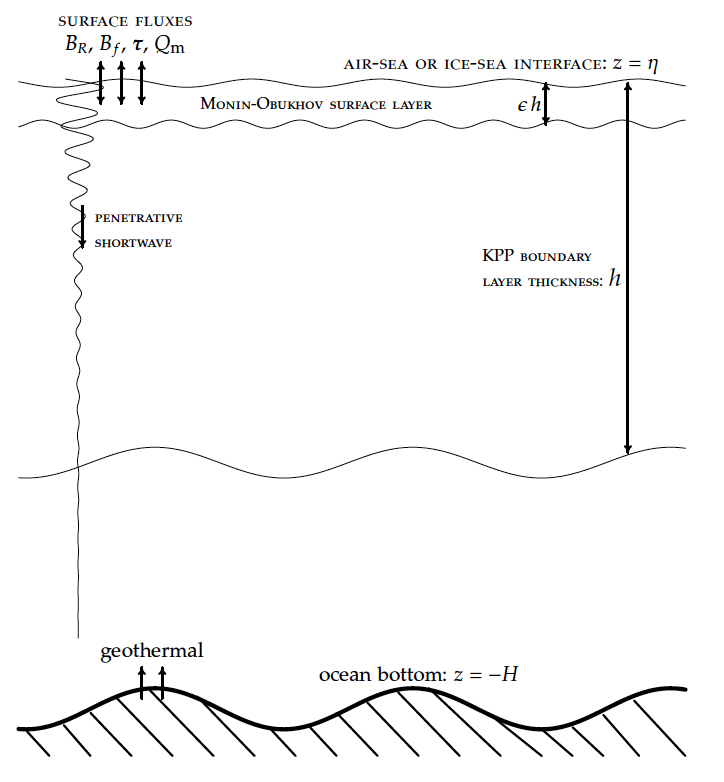
\includegraphics[width=3in]{figures/Figure81_CVmix_manual.png}
  \caption{Figure and caption (modified) from \cite{Griffies2015b}: ``Schematic of the upper ocean boundary layer regions associated with the KPP boundary layer parameterisation. The upper ocean is exposed to non-penetrative air-sea and ice-sea fluxes of momentum, mass $Q_m$, and buoyancy $B_f$. In addition, there is penetrative shortwave radiation, indicated by the exponentially decaying vertical sinusoidal. The Monin-Obukhov surface layer has a thickness 0.1$h$. The surface layer is where turbulence delivers fluxes to the molecular skin layer for transfer to the atmosphere or ice. The surface layer starts from just beneath the surface roughness elements at the upper ocean interface. Since neither these roughness elements, nor the molecular viscous sublayer, are resolved in ocean models, we assume in practice that the Monin-Obukhov surface layer extends to the sea surface at $z(x,y,t)$. The KPP boundary layer includes the surface layer, and it has a thickness $h(x,y,t)$ determined by the KPP parameterisation. The ocean bottom at $z(x,y)$ is rigid and is exposed to geothermal heating.''}% \textcolor{red}{[Navid: is there a typo in the red? $z=(x,y)$? ]}}
\end{figure}

\subsection{Air-sea fluxes}

The total net surface heat flux ($Q_{AS}$) into the ocean results from the interaction of radiative and turbulent fluxes:
\begin{equation}
    Q_{AS} = Q_{S} + Q_{L} +  \boldsymbol{\tau} + E + Q_{E} + Q_{H},
\end{equation}
where the radiative fluxes comprehend the shortwave solar radiation ($Q_{S}$) and net surface longwave solar radiation ($Q_{L}$). The shortwave radiation is computed from the solar insolation $Q_{I}$ incident on the ocean surface subtracted from the portion reflected from the ocean surface:
\begin{equation}
    Q_{S} = Q_{I}(1 - \alpha),
\end{equation}
with $\alpha$ being the albedo, a function of the clouds and usually with a value of 0.065 for the ocean \citep{Payne1972}. The net surface longwave solar is defined by:
\begin{equation}
    Q_{L} = Q_{A} - \sigma_{\text{SB}} , \mathrm{SST}_{\text{skin}}^{4},
\end{equation}

where $Q_{A}$ is the downwelling longwave flux from the atmosphere, $\sigma_{\text{SB}} = 5.67\times10^{-8}\,\text{W}\,\text{m}^{-2}\,\text{K}^{-4}$ is the Stefan-Boltzmann constant.

The turbulent fluxes include contribution from both latent and sensible heat exchange, which includes the wind stress ($\tau$), %[Navid: I don't understand what this means]
evaporation ($E$), latent heat ($Q_{E}$) and sensible heating ($Q_{H}$), defined by:
\begin{align}
    \boldsymbol{\tau} &= \rho C_{D} \left( \zeta_{10} \right) |\Delta \boldsymbol{U}| \Delta \boldsymbol{U}, \\
    E &= \rho C_{E} \left( \zeta_{10} \right) | q - q_{s} \left( SST \right)| |\Delta \boldsymbol{U}|, \\
    Q_{E} &= \Lambda_{V} E, \\
    Q_{H_{sens}} &= \rho c_{p} C_{H} \left( \zeta_{10} \right) \left( \Theta - SST \right) |\Delta \boldsymbol{U}|.
\end{align}
%{\color{red}[Navid: 1. Ιs there a typo in eq. (20.5)? There are three $|$.\\ 2. Why is $\tau$ bold in eq. (20.4) but not in eq. (20.1)? Is there a typo?]}

These fluxes are parameterised using the Bulk formulae \citep{Large2008} from the near surface atmospheric state (meridional and zonal components of the wind $\boldsymbol{U}$, potential temperature $\Theta$, specific humidity $q$ and density $\rho$) %[Navid: what are all these? Are these introduced to be used in eqs. (20.4-20.7)? If so, you should defined them after those eqs.] 
and the surface ocean state (SST and surface ocean currents). While CORE and JRA-55-do provided the atmospheric state, the ocean state are usually taken from the surface ocean model grid cell. At the time of the CORE bulk formulae was developed, it was considered an ocean model upper-layer of around 10~$m$; as the use of models with higher resolution become more common, a change in the bulk formulae might be required.
%{\color{Green}While CORE and JRA-55-do provided the atmospheric state, the ocean state are usually taken from the surface ocean model grid cell, which is an appropriated choice since the Bulk formulae was developed for the upper-ocean (around 10~$m$ for climate models, which have to be take in account when running a model with higher vertical resolution). \textcolor{red}{[Navid: Again a long sentence that confused me.]}} The turbulent fluxes are defined by:

The dimensionless atmospheric stability ($\zeta_{10}$) uses a reference height of 10~$m$, the specific heat capacity of air is given by $c_{p} \approx 1000.5 \text{J}\,\text{kg}$, $\Lambda_{V} = 2.5 \times 10^{6} \text{J}\,\text{kg}$ is the latent heat of vaporisation for water and the difference between the atmospheric winds and ocean currents is defined by $\Delta \boldsymbol{U} = \boldsymbol{U} - \boldsymbol{U}_{0}$ \citep{Pacanowski1987}.

The methodology for shifting the neutral 10~$m$ transfer coefficients for drag ($C_{D}$), sensible heat exchange ($(C_{h}$) and evaporation ($C_{E}$) are defined in \cite{Large2004}. Following the CORE-I study in \cite{Griffies2009}, most of the ocean is cooled by negative $Q_{H}$ and $Q_{E}$, which makes $\zeta_{10}$ negative and the atmosphere unstable. The majority of models in the \cite{Griffies2009} study computed incorrect transfer coefficients and have a fractional error associated, which is usually greater than unity and larger in regions where high SST and low winds speeds are combined to make a significantly unstable atmosphere. In addition, where these regions experienced significant surface cooling through latent heat flux there are an intensification of the error due to the loss, which makes the heat flux error larger.

\subsection{Boundary layer scheme}

In the 1-dimensional vertical scheme, the time-evolution of a tracer $\bar{\Lambda}$ is:
\begin{equation}
    \frac{\partial \bar{\Lambda}}{\partial t} = \frac{\partial(\overline{w \lambda})}{\partial z} - \frac{\partial \overline{w' \lambda '}}{\partial z},
\end{equation}

where the first term in RHS represents the resolved advection and the second term is the turbulent (subgridscale) correlation. {\color{red}[Navid: What's the overline?]}. {\color{red}The subscrid scale turbulent fluxes need} to be parameterised:
\begin{equation}
    \overline{w' \lambda '} = \overline{w \lambda}^{\text{local}} + \overline{w \lambda}^{\text{non-local}}.
\end{equation}

The turbulent correlation is parameterised as a the local and a  non-local term. The local term is the familiar downgradient diffusion:
\begin{equation}
     \overline{w \lambda}^{\text{local}} = -K \frac{\partial \bar{\Lambda}}{\partial z},
\end{equation}
with $K$ the turbulent diffusion coefficient. The non-local term is given by:
\begin{equation}
    \overline{w \lambda}^{\text{non-local}} = K^{\text{non-local}} \, \gamma,
\end{equation}
where $\gamma$ is the non-local term, which comes from a remotely place in the vertical. An example of the non-local effect is under a negative surface buoyancy forcing, which triggers instabilities that will propagate downward in the ocean boundary layer. The $K^{\text{non-local}}$ is function of a turbulent velocity scale $w$ and a structure function $G$, both only function of the depth $z$:
\begin{equation}
    K^{\text{non-local}} = h \, w(z) \, G(z).
\end{equation}

The depth of the boundary layer is often defined in function of the Bulk Richardson number:
\begin{equation}
    Ri(d) = \frac{(d-d_{r}) \left[ B_{r} - B(d) \right]}{| \boldsymbol{U}_{r} - \boldsymbol{U}(d) |^{2}} + U^{2}_{z},
\end{equation}
where $\boldsymbol{U}(d)$ is the horizontal velocity and $B(d)$ buoyancy at depth $d$ and $B_{r}$ and $\boldsymbol{U}_{r}$ within the Monin-Obukhov surface layer (see Fig \ref{cvmix_fig8.1}). The Richardson critical number ($Ri_{crit}$) is usually defined between 0.25 and 0.3 - which is a tuning parameter of ocean models. Then we can define:
\begin{align*}
    Ri(d) < Ri_{crit} \textrm{ if is within the boundary layer;}\\
    Ri(d) > Ri_{crit} \textrm{ if is outside the boundary layer.}
\end{align*}
% !TEX root = main.tex

\section{Lecture 21: Advection Schemes and Numerical Diffusion}
\begin{flushright}\textbf{[by Ryan Holmes]}\end{flushright}

In this lecture we took an introductory look at numerical advection
schemes and examined some of their basic properties and issues.

Consider the one-dimensional advection equation,
\begin{equation}
\frac{\partial\Theta}{\partial t} = -u \frac{\partial\Theta}{\partial x},\label{L21:ADE}
\end{equation}
where $\Theta(x,t)$ is a tracer and $u$ is a \textit{positive}
constant. A solution can be easily written down,
\begin{equation}
\Theta(x,t) = \Theta_0(x-ut),\label{L21:ADEsol}
\end{equation}
where $\Theta_0(x)$ is the tracer distribution at the initial time
$t=0$. In other words, the initial tracer distribution should
translate toward the positive $x$ direction without changing
shape. Note that throughout this lecture we will ignore the influence
of boundary conditions on $x$ (although these can easily be
incorporated).

We now consider solving Eq. \eqref{L21:ADE} on a discrete grid using
finite differences, to see how a numerical solution may differ from
the known analytic solution Eq. \eqref{L21:ADEsol}. We discretize
Eq. \eqref{L21:ADE} onto a regularly spaced grid $x_i$
($i\in 1,\cdot\cdot\cdot N$) with grid spacing $\Delta x$ and with a
regular time step $\Delta t$ such that the discrete time vector is
given by $t^k$ ($k\in 0,\cdot\cdot\cdot M$). $\Theta_i^k$ denotes the
value of the tracer at location $x_i$ and time $t^k$.

We will first examine the \textbf{forward-time, backward-space}
discretization of Eq. \eqref{L21:ADE},
\begin{equation}
  \frac{\Theta_i^{k+1}-\Theta_i^k}{\Delta t} = -u
  \frac{\Theta_i^k-\Theta^k_{i-1}}{\Delta x}.\label{L21:FTBS}
\end{equation}
Here we have discretized the time derivative with a forward
difference and the space derivative with a backward difference. This
equation is easy to time step forward by rearranging to determine the tracer
concentration at time step $k+1$ from the tracer concentration at time
step $k$,
\begin{equation}
  \Theta_i^{k+1} = -\frac{u\Delta t}{\Delta x}\left(\Theta_i^k-\Theta^k_{i-1}\right)+\Theta_i^k.\label{L21:EXTS}
\end{equation}

How does Eq. \eqref{L21:FTBS} differ from the continuous version
Eq. \eqref{L21:ADE}? To answer this question we employ \textbf{Hirt's
  Stability Analysis}. Each term in Eq. \eqref{L21:FTBS} is written in
terms of a Taylor expansion about $\Theta_i^k$. I.e.,
\begin{align}
  \Theta_i^{k+1} &= \Theta_i^k+\Delta t\frac{\partial\Theta}{\partial
  t}\Big|_i^k+\frac{(\Delta t)^2}{2}\frac{\partial^2\Theta}{\partial
  t^2}\Big|_i^k + \mathcal{O}((\Delta t)^3), \\
  \Theta_{i-1}^k &= \Theta_i^k-\Delta x\frac{\partial\Theta}{\partial
  x}\Big|_i^k+\frac{(\Delta x)^2}{2}\frac{\partial^2\Theta}{\partial
  x^2}\Big|_i^k + \mathcal{O}((\Delta x)^3).
\end{align}
Substitution of these forms into Eq. \eqref{L21:FTBS}, followed by
some tedious rearrangement (This is left as an exercise --- note that one must use the continuous form Eq. \eqref{L21:ADE} to convert the remaining
time derivatives into spatial derivatives) yields,
\begin{equation}
  \frac{\partial\Theta}{\partial t} = -u
  \frac{\partial\Theta}{\partial x} + \frac{u}{2}\left(\Delta
    x-u\Delta t\right)\frac{\partial^2\Theta}{\partial x^2} +
  \mathcal{O}\left((\Delta x)^2,\Delta x\Delta t,(\Delta t)^2\right),\label{L21:FTBSepde}
\end{equation}
Eq. \eqref{L21:FTBSepde} is known as the \textbf{modified equivalent
  PDE for the FTBS scheme}.

Comparing this modified PDE to our original continuous PDE
[Eq. \eqref{L21:ADE}] shows that the finite difference discretization
results in a leading order error term proportional to
$\frac{\partial^2\Theta}{\partial x^2}$ - i.e. a diffusive correction
term.  We set out to solve an advection equation, but by the act of
discretizing the equation using finite differences we have in fact
ended up with an advection--diffusion equation. The coefficient in
front of the leading order error term can be thought of as a
\textbf{numerical diffusivity},
\begin{equation}
  \kappa_{num} = \frac{u}{2}\left(\Delta x-u\Delta t\right).\quad\text{ FTBS}\label{L21:FTBSKnum}
\end{equation}
If $\kappa_{num}>0$ then the diffusion is down-gradient, resulting in
the weakening of any sharp gradients in the tracer field through
\textbf{numerical diffusion}. 

However, $\kappa_{num}$ is not guaranteed to be positive. If
$\kappa_{num}$ is negative, then the leading-order correction term
drives up-gradient diffusion (or \textit{un-mixing}) which acts to
increase gradients. Since the rate at which gradients are increased
depends on the gradients themselves, this can result in exponential
growth and the solution becomes unstable. Introducing the
\textbf{Courant} number,
\begin{equation}
  C = \frac{u\Delta t}{\Delta x},
\end{equation}
the FTBS numerical diffusivity Eq. \eqref{L21:FTBSKnum} can be
rewritten as,
\begin{equation}
  \kappa_{num} = \frac{(\Delta x)^2}{2\Delta t}C(1-C).
\end{equation}
Therefore the FTBS scheme is stable if the Courant number is in the
range $0\leq C\leq 1$. Physically, this condition can be interpreted
in terms of the \textit{cone of influence} of the backward in space
operator. For the simple advection equation Eq. \eqref{L21:ADE} the
solution propagates along characteristics defined by $x=ut$. If this
information propagates across a grid cell in less than a time step
(corresponding to $C>1$), then the solution becomes unstable as the
value $\Theta_i^{k+1}$ cannot be determined from the values
$\Theta_{i-1}^k$ and $\Theta_i^k$ (if $C=1.5$ then we would need to
utilize $\Theta_{i-2}^k$ and $\Theta_{i-1}^k$, XXX: Draw a diagram to
illustrate this). 

The FTBS scheme is only stable when the velocity is positive $u>0$
(again because for $u<0$ the cone of influence of the backward in
space operator does not match the characteristics $x=ut$ of the
solution). This corresponds to an \textit{upwind} advection scheme. If
$u$ was instead negative, the forward-time, forward-space scheme
(FTFS) would be stable (providing $|C|<1$). If the sign of $u$ varies
throughout the domain one could choose to use a forward or a backward
spatial finite difference depending on the sign of $u$ (known as an
\textit{upwind} advection scheme).

What about the case $C=1$? With
$C=1$, $\kappa_{num}=0$ and in fact all of the error terms are
identically zero. This corresponds to the case where the solution
propagates exactly one grid cell with each time step, and thus
the discretized solution is exact. However, it is only
possible to have $C=1$ at every location if the velocity is constant.

What about centered differences in space? The \textit{forward time,
  centered space} (FTCS) discretization of Eq. \eqref{L21:ADE} is,
\begin{equation}
  \frac{\Theta_i^{k+1}-\Theta_i^k}{\Delta t} = -u
  \frac{\Theta_{i+1}^{k}-\Theta^k_{i-1}}{2\Delta x}.\label{L21:FTCS}
\end{equation}
The corresponding modified equivalent PDE is,
\begin{equation}
  \frac{\partial\Theta}{\partial t} = -u
  \frac{\partial\Theta}{\partial x} - \frac{u^2\Delta t}{2}\frac{\partial^2\Theta}{\partial x^2} +
  \mathcal{O}\left((\Delta x)^2,\Delta x\Delta t,(\Delta
    t)^2\right).\quad\text{ equivalent PDE for FTCS}\label{L21:FTCSepde}
\end{equation}
In this case the numerical diffusivity,
\begin{equation}
  \kappa_{num} = -\frac{u^2\Delta t}{2},
\end{equation}
is always negative and thus the FTCS is unstable for any chosen time
step. One could stabilize schemes such as this by adding explicit
diffusion to the solution with a diffusivity that exceeds the
numerical diffusivity (e.g. a term
$\kappa_p\frac{\partial^2\Theta}{\partial x^2}$ to Eq. \eqref{L21:ADE},
where $\kappa_p>\kappa_{num}$). In the FTCS case such a scheme is
known as the \textit{Lax-Wendroff} scheme.

So far we have considered only forward time-stepping schemes. These
are known as \textit{explicit} in time, and are computationally easy
to time step as they can be written in the form of
Eq. \eqref{L21:EXTS}, where all of the RHS terms are known at the
current time and thus the tracer field at the next time step is easy
to determine. An example of an \textit{implicit} scheme is the
\textit{backward time, backward space} (BTBS) scheme,
\begin{equation}
  \frac{\Theta_i^{k}-\Theta_i^{k-1}}{\Delta t} = -u
  \frac{\Theta_i^{k}-\Theta^k_{i-1}}{\Delta x}.\label{L21:BTBS}
\end{equation}
The corresponding modified equivalent PDE for BTBS is,
\begin{equation}
  \frac{\partial\Theta}{\partial t} = -u
  \frac{\partial\Theta}{\partial x} + \frac{u}{2}\left(\Delta x + u
    \Delta t\right)\frac{\partial^2\Theta}{\partial x^2} +
    \mathcal{O}\left((\Delta x)^2,\Delta x\Delta t,(\Delta
      t)^2\right).\quad\text{ equivalent PDE for BTBS}\label{L21:FTCSepde}
\end{equation}
In this case the numerical diffusivity,
\begin{equation}
  \kappa_{num} = \frac{u}{2}\left(\Delta x + u\Delta t\right),
\end{equation}
is stable for any $u$ providing that we choose a large enough time
step. I.e. there is no upper time step stability restriction (or
Courant condition) on the BTBS scheme. However, for this implicit
scheme the solution is more difficult to time step, as the RHS of
Eq. \eqref{L21:BTBS} is evaluated at time level $k$ when only time
level $k-1$ is known. To solve Eq. \eqref{L21:BTBS} for the new time
level $k$ we rewrite it as a matrix equation,
\begin{equation}
  A_{ij}\Theta_j^k = \Theta_i^{k-1},\label{L21:BTBSmat}
\end{equation}
where
$A_{ij} = (1+\frac{u\Delta t}{\Delta x})\delta_{ij} - \frac{u\Delta
  t}{\Delta x}\delta_{(i-1)j}$. Eq. \eqref{L21:BTBSmat} can then be
solved by matrix inversion, but at considerably more cost than the
simple forward time-stepping schemes considered above.

Finally, we consider the \textit{centered-time, centered-space} (CTCS)
scheme (centered-time time stepping is also known as leapfrog),
\begin{equation}
  \frac{\Theta_i^{k+1}-\Theta_i^{k-1}}{2\Delta t} = -u
  \frac{\Theta_{i+1}^{k}-\Theta^k_{i-1}}{2\Delta x}.\label{L21:CTCS}
\end{equation}
The corresponding modified equivalent PDE for CTCS is,
\begin{equation}
  \frac{\partial\Theta}{\partial t} = -u
  \frac{\partial\Theta}{\partial x} - \frac{u(\Delta x)^2}{6}(1-C^2)\frac{\partial^3\Theta}{\partial x^3} +
  \mathcal{O}\left((\Delta x)^3,(\Delta x)^2\Delta t,...\right).\quad\text{ equivalent PDE for CTCS}\label{L21:CTCSepde}
\end{equation}
This scheme is second-order accurate and the leading-order error term
now depends on the third-derivative of $\Theta$. This is known as a
\textit{dispersive} advection scheme, as the third-order derivative
causes different wave-number components of the solution to propagate
at different speeds (Exercise: write $\Theta$ in terms of its Fourier
series in $x$ and substitute into Eq. \eqref{L21:CTCSepde}, retaining only
the leading-order error term. You will find that the third-order
derivative modifies the propagation speed of the solution so that it
is no longer equal to $u$, and is dependent on
wave-number). Dispersive advection schemes can develop oscillations as
a result of this dispersion, or separation of different wave-number components
(a good example to consider is where $\Theta_0$ is a step
function). Dispersive advection schemes are often combined with
\textit{flux limiters} which prevent this development of extrema in
the tracer distribution.

For more information see \citet{Lomax2001}.

% !TEX root = main.tex

\section{Lecture 22: Title goes here}
\begin{flushright}\textbf{[by ????]}\end{flushright}



% !TEX root = main.tex

\section{Lecture 23: Title goes here}
\begin{flushright}\textbf{[by ????]}\end{flushright}



% !TEX root = main.tex

\section{Lecture 24: Title goes here}
\begin{flushright}\textbf{[by ????]}\end{flushright}
% please write the title only when you start writing the notes
% this way I know by glancing the table of contents where to look
% cheers, Navid

%Ok, thanks! Denise

%hi Zhi, I will start writing my notes and we can adding explanations and tidying things up as we go...

%In this lecture we derive the key equation for the water mass transformation (WTM), a process described in Groeskamp et al., 2019 as ``the mass transport of sea water through a surface with a constant propery value". Based on the tools learnt through this course we should be able to use a few approximations to calculate transformation in a model.

\include{lecture25}


\bibliographystyle{plainnat}
\bibliography{references}
\end{document}
